\documentclass[11pt,a4paper,oneside]{report}

\usepackage[utf8]{inputenc}
\usepackage[T1]{fontenc}
\usepackage{lmodern}
\usepackage{amsmath}
\usepackage[a4paper,margin=2.6cm]{geometry}
\usepackage{microtype}
\usepackage{xcolor}
\usepackage{graphicx}
\usepackage{booktabs}
\usepackage{tabularx}
\usepackage{enumitem}
\usepackage{caption}
\usepackage{fancyhdr}
\usepackage{listings}
\usepackage{tikz}
\usepackage{pgfplots}
\pgfplotsset{compat=1.17}
\usetikzlibrary{arrows.meta,positioning,shapes.geometric,fit,calc,backgrounds,decorations.pathreplacing}
\usepackage[hidelinks,colorlinks=true,linkcolor=blue!50!black,urlcolor=blue!50!black,citecolor=blue!50!black]{hyperref}

\setlist{itemsep=2pt,topsep=4pt}
\setlength{\parindent}{0pt}
\setlength{\parskip}{6pt}
\captionsetup{font=small,labelfont=bf}

\pagestyle{fancy}
\fancyhf{}
\fancyhead[L]{\small\nouppercase{\leftmark}}
\fancyfoot[C]{\thepage}
\renewcommand{\headrulewidth}{0.3pt}

\definecolor{codebg}{RGB}{247,247,250}
\definecolor{kw}{RGB}{0,70,140}
\definecolor{cm}{RGB}{90,110,90}
\definecolor{strc}{RGB}{150,50,50}

\lstdefinestyle{ckern}{
  language=C,
  basicstyle=\ttfamily\footnotesize,
  keywordstyle=\color{kw}\bfseries,
  commentstyle=\color{cm}\itshape,
  stringstyle=\color{strc},
  backgroundcolor=\color{codebg},
  frame=single,
  rulecolor=\color{black!20},
  numbers=none,
  breaklines=true,
  breakatwhitespace=false,
  columns=fullflexible,
  keepspaces=true,
  showstringspaces=false,
  tabsize=4,
  xleftmargin=4pt,
  xrightmargin=4pt,
  aboveskip=8pt,
  belowskip=6pt,
  morekeywords={u8,u16,u32,u64,bool,__user,__init,__exit,uint8_t,uint16_t,uint32_t,size_t,ssize_t}
}
\lstdefinestyle{shell}{
  language=sh,
  basicstyle=\ttfamily\footnotesize,
  keywordstyle=\color{kw}\bfseries,
  commentstyle=\color{cm}\itshape,
  stringstyle=\color{strc},
  backgroundcolor=\color{codebg},
  frame=single,
  rulecolor=\color{black!20},
  breaklines=true,
  columns=fullflexible,
  keepspaces=true,
  showstringspaces=false,
  xleftmargin=4pt,
  xrightmargin=4pt,
  aboveskip=8pt,
  belowskip=6pt
}
\lstset{style=ckern}

\newcommand{\code}[1]{\texttt{\small #1}}
\newcommand{\proj}{\textsc{bbcrypto}}

\tikzset{
  box/.style={draw=black!70,rounded corners=2pt,thick,minimum height=8mm,align=center,font=\small,fill=white},
  layer/.style={draw=black!70,rounded corners=2pt,thick,minimum height=9mm,minimum width=9.2cm,align=center,font=\small},
  arr/.style={-{Stealth[length=2.2mm]},thick},
  darr/.style={{Stealth[length=2.2mm]}-{Stealth[length=2.2mm]},thick},
  lbl/.style={font=\scriptsize,fill=white,inner sep=1pt}
}

\title{\textbf{Linux Device Drivers and the \proj{} Project}\\[6pt]
\large A USB crypto accelerator for the Linux kernel crypto API,\\
built on a BeagleBone Black}
\author{Aman Pathak}
\date{November 2026}

\begin{document}

\maketitle

\begin{abstract}
\noindent
This report has two parts. The first part explains how device drivers work in Linux. It covers the split between user space and the kernel, the device model, kernel modules, concurrency and memory rules in kernel code, the USB subsystem, the kernel crypto API, and the USB gadget side that lets a small computer pretend to be a USB device.
The second part describes a driver built with those ideas. A BeagleBone Black connects to a PC over USB. A kernel module on the PC registers hash, cipher and authenticated encryption algorithms with the Linux crypto API. Every operation is sent over a USB bulk pipe to a daemon on the board, which runs it on the board's AM335x hardware crypto engines. The report covers the wire protocol, the asynchronous command engine in the module, the board daemon, the build and deployment path, the test results, and the problems met along the way.
\end{abstract}

\tableofcontents
\listoffigures
\listoftables

% ====================================================================
\chapter{Introduction}
% ====================================================================

\section{Motivation}

A computer is more than its processor. Disks, network cards, keyboards, displays and accelerators all sit behind small pieces of software that translate between a general kernel interface and one particular piece of hardware. These pieces are device drivers. In Linux they make up the largest part of the kernel source tree, and writing one is the standard way to learn how the kernel is organised.

The aim of this project was to write a complete driver for a device that does not exist as a product. A BeagleBone Black is a small ARM board. Its AM335x processor contains hardware engines for AES and for the SHA family. The board can also present itself to a PC as a USB device. The project connects the two ideas. The PC sees a USB peripheral, loads a driver for it, and from then on the board's crypto engines are available to every program on the PC through the ordinary kernel crypto interface.

\section{What was built}

The result has two programs and one shared header.

\begin{itemize}
  \item \textbf{A kernel module on the PC} (\code{host/bbcrypto.c}). It is a USB driver. When the board is plugged in, the module binds to it, then registers algorithms with the kernel crypto API: \code{sha1}, \code{sha256}, \code{hmac(sha256)}, \code{ecb(aes)}, \code{cbc(aes)}, \code{ctr(aes)} and \code{gcm(aes)}.
  \item \textbf{A daemon on the board} (\code{board/bbcryptod.c}). It exposes a vendor specific USB interface through FunctionFS, reads requests from the PC, executes them through the board's own kernel (which uses the AM335x hardware), and sends replies.
  \item \textbf{A protocol header} (\code{proto.h}) included by both sides, so the message layout is defined once.
\end{itemize}

Around those sit a test suite with 690 checks, a command line tool, eleven demonstration programs, deployment scripts for a remote machine, and service files for the board.

\section{How to read this report}

Chapters~\ref{ch:kernel} to~\ref{ch:gadget} are general. A reader who already knows Linux driver programming can skip to Chapter~\ref{ch:design}. Chapters~\ref{ch:design} to~\ref{ch:board} describe the design and the code in detail. Chapter~\ref{ch:tools} covers the tools, demonstrations and operation, Chapter~\ref{ch:build} building and deployment, Chapter~\ref{ch:test} the testing and measurements, Chapter~\ref{ch:lessons} the problems met, and Chapter~\ref{ch:security} the security considerations. A glossary and a bibliography close the report. Source files are referred to by their path in the repository.

% ====================================================================
\part{How Linux drivers work}
% ====================================================================

\chapter{The kernel and its drivers}\label{ch:kernel}

\section{User space and kernel space}

Linux separates code into two privilege levels. Programs run in \emph{user space}. They cannot touch hardware, cannot read each other's memory, and can only ask the kernel to act for them through \emph{system calls}. The kernel runs in \emph{kernel space} with full access to memory and devices. A driver is kernel code, so a bug in a driver can crash the whole machine or corrupt memory belonging to any process. That is why drivers are written in a defensive style, with every error path handled and every resource counted.

Figure~\ref{fig:layers} shows the layers a request passes through. A program calls a system call such as \code{read}, \code{write}, \code{ioctl} or \code{sendmsg}. The \emph{virtual file system} or another subsystem routes the call to the right kernel component. That component may be a driver, which then talks to hardware.

\begin{figure}[ht]
\centering
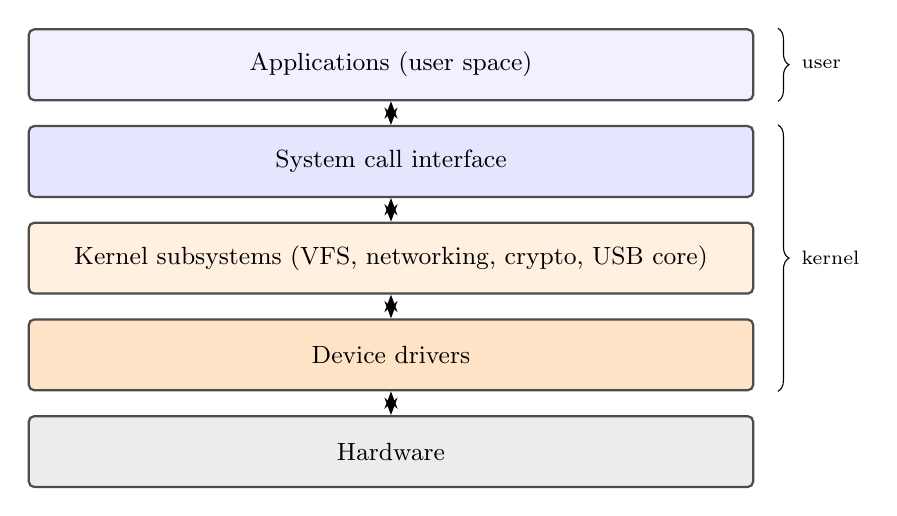
\begin{tikzpicture}[node distance=3mm]
  \node[layer,fill=blue!6] (app) {Applications (user space)};
  \node[layer,fill=blue!10,below=of app] (sys) {System call interface};
  \node[layer,fill=orange!12,below=of sys] (sub) {Kernel subsystems (VFS, networking, crypto, USB core)};
  \node[layer,fill=orange!22,below=of sub] (drv) {Device drivers};
  \node[layer,fill=gray!15,below=of drv] (hw) {Hardware};
  \foreach \a/\b in {app/sys,sys/sub,sub/drv,drv/hw} \draw[darr] (\a) -- (\b);
  \draw[decorate,decoration={brace,amplitude=4pt}] ([xshift=3mm]app.north east) -- ([xshift=3mm]app.south east) node[midway,right=5pt,font=\scriptsize]{user};
  \draw[decorate,decoration={brace,amplitude=4pt}] ([xshift=3mm]sys.north east) -- ([xshift=3mm]drv.south east) node[midway,right=5pt,font=\scriptsize]{kernel};
\end{tikzpicture}
\caption{Layers between a program and a device.}\label{fig:layers}
\end{figure}

\section{What a driver is}

A driver is the part of the kernel that knows one kind of hardware. It has two faces.

\begin{itemize}
  \item \textbf{Towards the hardware} it knows registers, interrupts, buses and protocols.
  \item \textbf{Towards the rest of the kernel} it implements an interface that a subsystem defines, so that the subsystem can treat all devices of one kind in the same way.
\end{itemize}

A block driver implements the block layer interface, a network driver implements the network device interface, and a character driver implements file operations. The driver in this project is unusual in one respect. It is a \emph{USB driver} towards the hardware, but towards the rest of the kernel it is a \emph{crypto algorithm provider}. It does not create a device node. Instead it adds entries to the crypto API's table of algorithms.

\section{Classes of drivers}

Linux traditionally describes three classes.

\begin{description}
  \item[Character devices] give a stream of bytes with \code{open}, \code{read}, \code{write} and \code{ioctl}. Serial ports, input devices and many sensors are of this class.
  \item[Block devices] transfer fixed size blocks and are used for storage. The block layer adds queuing and caching above them.
  \item[Network interfaces] send and receive packets. They do not appear as files but as interfaces managed through sockets.
\end{description}

Many drivers do not fit one class cleanly. USB drivers sit on top of the USB core and may then present themselves as any class, or as a provider for another subsystem as in this project.

\section{Loadable modules}

Most drivers are built as \emph{loadable kernel modules}. A module is an object file with the suffix \code{.ko}. It is linked into the running kernel with \code{insmod} or \code{modprobe} and removed with \code{rmmod}. Two functions mark its life.

\begin{lstlisting}
static int __init bbc_init(void)
{
	int ret;

	bbc_wq = alloc_ordered_workqueue("bbcrypto", WQ_MEM_RECLAIM);
	if (!bbc_wq)
		return -ENOMEM;
	ret = usb_register(&bbc_driver);
	if (ret)
		destroy_workqueue(bbc_wq);
	return ret;
}

static void __exit bbc_exit(void)
{
	usb_deregister(&bbc_driver);
	bbc_unregister_algs();
	destroy_workqueue(bbc_wq);
}

module_init(bbc_init);
module_exit(bbc_exit);
\end{lstlisting}

The init function runs when the module loads. It allocates what the driver needs globally and registers with the subsystem. If anything fails it must undo what it already did and return a negative error number. The exit function undoes everything in reverse order. The same listing from the project shows the pattern: allocate a workqueue, register the USB driver, and on failure release the workqueue.

A module declares metadata with macros: \code{MODULE\_LICENSE("GPL")} matters because several kernel interfaces are only exported to GPL compatible modules. \code{MODULE\_DEVICE\_TABLE} writes the list of devices a driver handles into the module, so that tools can load the module automatically when matching hardware appears.

\paragraph{Module parameters.} A module can take settings at load time and, if the permission bits allow it, change them at run time through \code{/sys/module/<name>/parameters/}. The project uses this for \code{prio}, \code{window} and \code{chunk}:

\begin{lstlisting}
static unsigned int prio = 50;
module_param(prio, uint, 0444);      /* read only after load */

static unsigned int window = 4;
module_param(window, uint, 0644);    /* can be changed while running */
\end{lstlisting}

\paragraph{Out of tree builds.} A module is built against the headers and configuration of one particular kernel. The build uses the kernel's own \emph{kbuild} system, driven by a two line Makefile (\code{obj-m := bbcrypto.o}). A module built for one kernel version will not load into another, because the module records the kernel version string and symbol checksums.

\section{Kernel programming rules}

Kernel code lives under tighter rules than user programs. Several of them shaped this project.

\paragraph{No standard library.} There is no \code{malloc}, \code{printf} or \code{pthread}. The kernel offers \code{kmalloc} and \code{kfree}, \code{printk} with the \code{dev\_err} family, and its own locking and threading primitives.

\paragraph{Allocation flags.} \code{kmalloc} takes a flag that says what the allocator may do. \code{GFP\_KERNEL} may sleep to reclaim memory. \code{GFP\_ATOMIC} may not sleep, and is required in interrupt context. \code{GFP\_NOIO} forbids starting disk input or output, which avoids deadlock when the allocation happens on the path that writes data to disk. The driver uses \code{GFP\_NOIO} when it submits a request on behalf of a crypto operation, so that a crypto request can never wait on disk input or output, which could deadlock if the request itself sits on a storage path.

\paragraph{Contexts and sleeping.} Code runs in one of several contexts. Process context belongs to a task and may sleep. Interrupt and softirq context may not sleep. A USB completion handler runs in interrupt (or softirq) context, so inside it the driver may only use spinlocks and non sleeping allocation, and anything that must sleep is handed off to a workqueue.

\paragraph{Locking.} Shared data is protected by locks. A \emph{spinlock} busy waits and can be taken in interrupt context, so it protects short critical sections. A \emph{mutex} sleeps and protects longer ones. The variant \code{spin\_lock\_irqsave} also disables local interrupts, which is needed when an interrupt handler takes the same lock. The driver's per board state is under one spinlock, and completion callbacks are never invoked while it is held.

\paragraph{Reference counting.} The lifetime of an object that several parties point to is managed with a \code{struct kref}. Each user takes a reference and drops it when done, and the last drop frees the object. This is how the driver stops a board structure from disappearing while a request still refers to it after the USB cable was pulled.

\paragraph{Deferred work.} Heavy or sleeping work is put on a \emph{workqueue}, which runs a function later in process context. The project uses one ordered workqueue so that its work items run one at a time, in order, and need less locking.

\paragraph{Errors are negative numbers.} Functions return \code{0} for success or a negative \code{errno} value such as \code{-ENOMEM} or \code{-ENODEV}. Asynchronous operations return \code{-EINPROGRESS} when they have been accepted and will finish later.

\section{The device model and sysfs}

The kernel keeps an internal tree of buses, devices and drivers, the \emph{device model}. Each bus type (PCI, USB, platform and so on) holds a list of devices and a list of drivers. When a new device appears the bus tries to match it with a driver, using an \emph{id table}, and on a match calls the driver's \code{probe} function. When the device goes away it calls \code{disconnect} (or \code{remove}). The tree is exported to user space as a file system, \emph{sysfs}, under \code{/sys}. A driver can add its own files there. This project adds two files below the USB interface directory: \code{stats} and \code{ping}.

\section{A minimal character driver for comparison}\label{sec:minchar}

Before the project's driver it helps to see the smallest useful driver, so that the pieces added later are recognisable. The listing below is illustrative and is not part of the project. It registers a character device that returns a fixed string.

\begin{lstlisting}
#include <linux/module.h>
#include <linux/fs.h>
#include <linux/miscdevice.h>
#include <linux/uaccess.h>

static ssize_t hello_read(struct file *f, char __user *buf,
			  size_t len, loff_t *pos)
{
	static const char msg[] = "hello\n";

	return simple_read_from_buffer(buf, len, pos, msg, sizeof(msg) - 1);
}

static const struct file_operations hello_fops = {
	.owner = THIS_MODULE,
	.read  = hello_read,
};

static struct miscdevice hello_dev = {
	.minor = MISC_DYNAMIC_MINOR,
	.name  = "hello",
	.fops  = &hello_fops,
};

module_misc_device(hello_dev);
MODULE_LICENSE("GPL");
\end{lstlisting}

Three things are visible even here. The driver fills a table of function pointers (\code{file\_operations}) that the kernel calls on behalf of user programs. It copies data across the privilege boundary with a dedicated helper (\code{simple\_read\_from\_buffer} uses \code{copy\_to\_user}), because a user pointer cannot be dereferenced directly. And it registers with a subsystem (here the misc device class) instead of creating device nodes by hand.

The \proj{} driver follows the same shape, with a bigger interface table: instead of \code{file\_operations} it fills \code{usb\_driver} for the bus side and \code{skcipher\_alg}, \code{shash\_alg}, \code{ahash\_alg} and \code{aead\_alg} for the crypto side.

\section{Interrupts and deferred work}

Hardware signals the processor with an \emph{interrupt}. The processor stops what it was doing, runs the registered \emph{interrupt handler}, and returns. Because every other activity on that processor waits while the handler runs, handlers must be short. The kernel splits interrupt work into two halves.

\begin{description}
  \item[Top half] runs immediately in interrupt context. It acknowledges the hardware, reads what it needs to, and schedules the rest.
  \item[Bottom half] runs later with interrupts enabled. The kernel offers several mechanisms: softirqs and tasklets (still atomic context, cannot sleep) and \emph{workqueues} (process context, can sleep).
\end{description}

A USB driver does not usually see a hardware interrupt. The host controller driver handles that, and calls the driver's URB completion function. That function runs in softirq context, so it is the driver's top half in practice. The project's completion handlers follow the rule strictly. They take a spinlock, move a command between lists, and queue a work item. The slow part (calling back into the crypto layer, copying data, building new commands) happens on the workqueue.

\begin{table}[ht]
\centering
\begin{tabularx}{\textwidth}{lXX}
\toprule
Context & May do & May not do \\
\midrule
Process (workqueue, system call) & sleep, \code{GFP\_KERNEL}, take mutexes, wait on a completion & nothing special \\
Softirq / URB completion & spinlocks, \code{GFP\_ATOMIC}, queue work, submit URBs & sleep, mutexes, \code{wait\_for\_completion} \\
Hard interrupt & very short work & everything above that takes time \\
\bottomrule
\end{tabularx}
\caption{What each execution context allows.}
\end{table}

The synchronous helper \code{bbc\_xfer} in the project waits on a completion, so it may only be called from process context. The project respects this: it is used by the hash functions (which run in the caller's context) and by probe, never from a URB completion.

\section{Memory, scatterlists and DMA}

Kernel memory is allocated in several ways. \code{kmalloc} returns physically contiguous memory suitable for DMA. \code{vmalloc} returns memory that is contiguous only virtually. Pages can be taken directly for large buffers. The crypto layer avoids assuming a buffer is contiguous: data is described by a \emph{scatterlist}, an array of (page, offset, length) entries that together form a logical buffer. A driver that wants a flat buffer copies in or out.

The project does exactly that. A request's source and destination scatterlists are copied into the flat command buffer with \code{sg\_pcopy\_to\_buffer} and back with \code{sg\_pcopy\_from\_buffer}. Both take an offset, which is how a chunk in the middle of a long request is read and written without copying the rest. This costs one extra copy per direction. A DMA aware driver would map the scatterlist for the device and avoid the copy, but USB transfers go through the host controller, and the extra copy is small next to the USB transfer time.

\section{Locking in more detail}

The driver uses three lock levels, always taken in the same order.

\begin{table}[ht]
\centering
\begin{tabularx}{\textwidth}{llX}
\toprule
Lock & Kind & Protects \\
\midrule
\code{bbc\_algs\_lock} & mutex & registration of the algorithms against board arrival and removal \\
\code{bbc\_reg\_lock} & spinlock & the global board list, device ids and the round robin pointer \\
\code{d->lock} & spinlock & everything about one board: the four command lists, counters of queued and in-flight commands, the \code{dead} flag \\
\bottomrule
\end{tabularx}
\caption{Locks of the host driver, outermost first.}
\end{table}

Two rules keep this simple. First, callbacks into the crypto layer are never made while a lock is held, because a callback can submit new requests and take the same lock again. Completed commands are first moved to a list under the lock, and a work item later runs their callbacks with no lock held. Second, only short, non sleeping things happen under a spinlock: list manipulation, counter updates, and the decision to send.

\section{Reference counts and object lifetime}

Table~\ref{tab:refs} lists what holds a reference to what. The \code{kref} pattern replaces explicit ownership: each holder takes a reference before use and releases it after, and the final release frees the object.

\begin{table}[ht]
\centering
\begin{tabularx}{\textwidth}{lXl}
\toprule
Object & Holders of a reference & Freed by \\
\midrule
board (\code{bbc\_dev}) & the USB interface data pointer, each queued work item, each command, the timer, each caller of \code{bbc\_get} & \code{bbc\_release} \\
command (\code{bbc\_cmd}) & the engine, each URB submission of it, a synchronous waiter & \code{bbc\_cmd\_free} \\
\bottomrule
\end{tabularx}
\caption{Reference holders.}\label{tab:refs}
\end{table}

\code{bbc\_kick} shows the pattern in four lines: it takes a reference on the board, tries to queue the work, and if the work was already queued (so it will run once anyway) drops the extra reference at once. The work function releases its reference when it ends. A board structure therefore cannot be freed while a work item that refers to it is pending.

\section{Tools for observing a driver}

A driver cannot be understood without looking at it running. The tools used during this project are standard.

\begin{table}[ht]
\centering
\begin{tabularx}{\textwidth}{lX}
\toprule
Tool & What it shows \\
\midrule
\code{dmesg} & kernel log: the driver's \code{dev\_info} and \code{dev\_err} lines, probe and disconnect messages, warnings from the crypto core \\
\code{lsusb -v}, \code{lsusb -t} & descriptors the device presents and the tree of devices and bound drivers \\
\code{/sys/bus/usb/drivers/bbcrypto/} & which interfaces are bound, and the driver's own files \code{stats} and \code{ping} \\
\code{/sys/module/bbcrypto/parameters/} & current values of \code{prio}, \code{window} and \code{chunk} \\
\code{/proc/crypto} & every registered algorithm with name, driver, priority, type and flags \\
\code{modinfo} & module metadata, parameters, vermagic \\
\code{lsmod}, \code{insmod}, \code{rmmod} & loaded modules, load and unload \\
\bottomrule
\end{tabularx}
\caption{Observation tools.}
\end{table}

The project adds one more on purpose: the \code{stats} file. Counters for requests, bytes, errors and retries let a test prove not only that an answer was right, but that it was computed on the board.

\section{Kernel versions and the missing stable interface}

User space has a stable binary interface; the kernel does not promise one for modules. Internal functions change between versions, headers move, and a module compiled for one kernel refuses to load into another because the module records a version string and symbol checksums (the \emph{vermagic} and \emph{modversions}). This has a practical consequence for the project: the module must be rebuilt for the kernel of the machine it runs on. That is why the deployment script builds on the target and does not copy a binary.


\chapter{USB from the driver's point of view}\label{ch:usb}

\section{The bus}

USB is a host controlled bus. One host, the PC, starts every transfer. Devices only answer. Devices hang from a tree of hubs, and each has an address assigned when it is enumerated. The host controller driver (xHCI on a modern PC) is part of the kernel and deals with the bus hardware. A device driver does not talk to it directly. It talks to the \emph{USB core}, which provides a uniform API.

\section{Descriptors}

When a device is plugged in, the host reads a set of \emph{descriptors} that describe it. They form a hierarchy (Figure~\ref{fig:desc}).

\begin{figure}[ht]
\centering
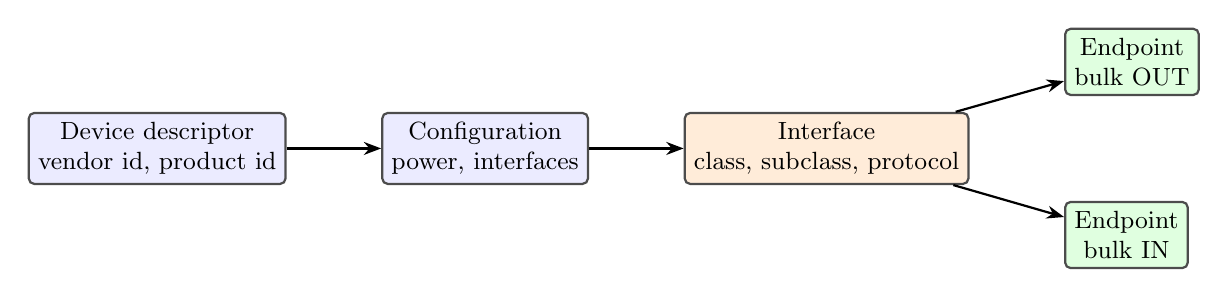
\begin{tikzpicture}[node distance=5mm and 12mm]
  \node[box,fill=blue!8] (dev) {Device descriptor\\vendor id, product id};
  \node[box,fill=blue!8,right=of dev] (cfg) {Configuration\\power, interfaces};
  \node[box,fill=orange!15,right=of cfg] (if) {Interface\\class, subclass, protocol};
  \node[box,fill=green!12,above right=2mm and 12mm of if] (e1) {Endpoint\\bulk OUT};
  \node[box,fill=green!12,below right=2mm and 12mm of if] (e2) {Endpoint\\bulk IN};
  \draw[arr] (dev) -- (cfg);
  \draw[arr] (cfg) -- (if);
  \draw[arr] (if) -- (e1);
  \draw[arr] (if) -- (e2);
\end{tikzpicture}
\caption{USB descriptor hierarchy as seen by the driver.}\label{fig:desc}
\end{figure}

A \emph{configuration} groups \emph{interfaces}. Each interface is one function of the device and is what a Linux driver binds to. An interface has \emph{endpoints}, which are the data pipes. Each endpoint has a direction (IN means device to host, OUT means host to device), a transfer type, and a maximum packet size.

\section{Transfer types}

\begin{table}[ht]
\centering
\begin{tabularx}{\textwidth}{lXl}
\toprule
Type & Purpose & Guarantee \\
\midrule
Control & configuration and commands, always on endpoint 0 & delivery, small \\
Bulk & large, loss free data when the bus has spare time & delivery, no timing \\
Interrupt & small data polled at a fixed rate & latency bound \\
Isochronous & streams such as audio & timing, no retry \\
\bottomrule
\end{tabularx}
\caption{USB transfer types.}
\end{table}

This project uses \emph{bulk} transfers. Bulk is the right choice for a transfer of tens of kilobytes where correctness matters and timing does not. On a high speed link a bulk packet carries up to 512 bytes. A bulk transfer ends with a packet shorter than the maximum, or with a zero length packet. The project's protocol relies on this rule and has one special case for it, described in Section~\ref{sec:pad}.

\section{The driver structure}

A USB driver describes itself to the USB core with a \code{struct usb\_driver}.

\begin{lstlisting}
static const struct usb_device_id bbc_ids[] = {
	{USB_DEVICE_AND_INTERFACE_INFO(0x1d6b, 0x0104,
		BBC_USB_CLASS, BBC_USB_SUBCLASS, BBC_USB_PROTO)},
	{}};
MODULE_DEVICE_TABLE(usb, bbc_ids);

static struct usb_driver bbc_driver = {
	.name = DRV,
	.probe = bbc_probe,
	.disconnect = bbc_disconnect,
	.id_table = bbc_ids,
};
\end{lstlisting}

The \emph{id table} says which devices the driver wants. The project matches on the vendor and product id of the Linux gadget composite device (\code{1d6b:0104}) \emph{and} on the interface class triple (\code{0xff}, \code{0x5c}, \code{1}). Matching on the interface triple is what makes the driver bind to the one vendor specific interface of the board, and leave the serial and network functions of the same composite device to other drivers.

\section{URBs}

Data moves with \emph{URBs}, USB request blocks. An URB describes one transfer: the pipe, a buffer, a length, and a completion function. The driver fills one with \code{usb\_fill\_bulk\_urb}, submits it with \code{usb\_submit\_urb}, and returns at once. Later the USB core calls the completion function, in interrupt context, when the transfer finished or failed.

\begin{lstlisting}
usb_fill_bulk_urb(c->urb, d->udev, d->pipe_out,
		  c->obuf, c->olen, bbc_out_complete, c);
usb_anchor_urb(c->urb, &d->anchor);
ret = usb_submit_urb(c->urb, GFP_NOIO);
\end{lstlisting}

This listing is the heart of the transmit path. The \emph{anchor} is a list that collects all URBs of one device, so that on disconnect they can be cancelled in one call with \code{usb\_kill\_anchored\_urbs}. Without it the driver would have to track every outstanding URB itself.

\section{Probe and disconnect}

\code{probe} runs when a matching interface appears. It finds the endpoints, allocates the per device structure, posts the receive URB, checks that the device answers, creates sysfs files and registers whatever it provides. \code{disconnect} runs when the device is removed, possibly in the middle of a transfer. It must stop all traffic, fail or finish every pending request, and release every resource. Both functions are covered for this project in Section~\ref{sec:probe}.

A subtle point is that \code{disconnect} can race with anything: a request may be submitted by a program at the moment the cable is pulled. A driver defends with a flag (the project uses \code{dead}) set under the same lock that protects its queues, and reference counts that keep the structure alive until the last user lets go.

\section{Enumeration step by step}

When a device is connected the following happens, and the driver only gets involved at the end.

\begin{enumerate}
  \item The hub notices a change on a port and reports it to the host.
  \item The host resets the port, which also tells it the device speed.
  \item The host reads the first 8 bytes of the device descriptor on endpoint 0 to learn the maximum packet size of the control endpoint, then assigns the device an address.
  \item The host reads the full device descriptor, then the configuration descriptor with all interface and endpoint descriptors, and the strings.
  \item The host selects a configuration with a \code{SET\_CONFIGURATION} request.
  \item The USB core creates a device object for the device and an object for each interface. For each interface the bus tries to find a driver whose id table matches.
  \item The matching driver's \code{probe} is called.
\end{enumerate}

On the board side, FunctionFS is where those descriptors originate. The daemon supplies the interface and endpoint descriptors, and the gadget core assembles them into the configuration the host reads. Nothing in the host-side driver needs to know that the other side is Linux.

\section{Matching: devices, interfaces and class codes}

A device descriptor has a class field, and so does each interface descriptor. Standard classes (mass storage, audio, HID, communications) have standard drivers. The value \code{0xff} means \emph{vendor specific}: no standard driver may claim it, and the vendor supplies one. The project's interface is class \code{0xff}, subclass \code{0x5c}, protocol \code{1}. The subclass and protocol numbers are arbitrary and chosen by the project. Matching on all three together with the vendor and product id makes the match very specific.

The board is a \emph{composite} device: one USB device that offers several interfaces, here serial, Ethernet and the project's function. Each interface can have its own driver. The host's CDC drivers take the serial and network interfaces and \code{bbcrypto} takes the vendor specific one, all at once, which is why the board stays reachable over SSH while it works as a crypto accelerator.

\section{Speeds and packet sizes}

\begin{table}[ht]
\centering
\begin{tabular}{lrr}
\toprule
Speed & Signalling rate & Bulk max packet \\
\midrule
Full speed & 12 Mbit/s & 64 bytes \\
High speed & 480 Mbit/s & 512 bytes \\
SuperSpeed & 5 Gbit/s & 1024 bytes \\
\bottomrule
\end{tabular}
\caption{USB speeds and bulk packet sizes.}
\end{table}

The board's controller is a USB 2.0 controller that can run at high speed, and the daemon writes both a full speed and a high speed descriptor set, with 512 byte bulk packets for the latter. The theoretical ceiling of 480 Mbit/s is 60 MB/s. The measured transport only throughput of the project (Chapter~\ref{ch:test}) is roughly 6.5 MB/s, about a tenth of that, which shows how much slower the board's controller and the daemon path are than the wire.

\section{What a bulk transfer looks like on the wire}

A bulk OUT transfer of $n$ bytes is split by the host controller into packets of the endpoint's maximum size. Each packet is acknowledged by the device. If the device cannot take a packet (no buffer is queued) it answers with a negative acknowledgment (NAK) and the host retries later. This is what the project's protocol relies on for flow control: the host does not need to know whether the daemon is busy.

The \emph{transfer} ends with a packet shorter than the maximum. Table~\ref{tab:bulk} shows lengths and the packets they produce on a high speed link.

\begin{table}[ht]
\centering
\begin{tabular}{rll}
\toprule
Message length & Packets & Ends with \\
\midrule
35 & 35 & short packet (ends the transfer) \\
511 & 511 & short packet \\
512 & 512 & full packet, \emph{needs} a zero length packet or padding \\
513 & 512 + 1 & short packet \\
1024 & 512 + 512 & full packet, same problem \\
\bottomrule
\end{tabular}
\caption{Bulk transfers and the short packet rule at 512 bytes.}\label{tab:bulk}
\end{table}

A zero length packet is legal USB, but support for it varies between controller drivers. The project avoids depending on it. Whenever a message is an exact multiple of 512 bytes, the sender appends one byte of padding, so the final packet is always short. In the code this is one line in the command builder:

\begin{lstlisting}
if (c->olen % 512 == 0)
	c->obuf[c->olen++] = 0; /* force a short final packet */
\end{lstlisting}

and the corresponding line in the daemon's reply builder, \code{if (len \% 512 == 0) ce->buf[len++] = 0}.

\section{URB status codes}

A completed URB carries a status. The handlers distinguish three kinds.

\begin{description}
  \item[0] success.
  \item[\code{-ENOENT}, \code{-ECONNRESET}, \code{-ESHUTDOWN}] the URB was cancelled or the device is gone. These are expected on disconnect. The receive handler returns without resubmitting.
  \item[anything else] a real transfer error, for example \code{-EPROTO}, \code{-EILSEQ} or \code{-EOVERFLOW}. The receive handler tolerates up to twenty consecutive errors and resubmits the URB, then gives up with a log message. A send error finishes the command with that status.
\end{description}

\section{Hotplug, udev and automatic loading}

When the USB core finds a new interface it emits a \emph{uevent} with a \code{MODALIAS} string that encodes the ids, for example \code{usb:v1D6Bp0104\ldots ic FF isc 5C ip 01}. The user space daemon \code{udev} passes this to \code{modprobe}, which looks it up in the alias table written by \code{depmod} from every module's \code{MODULE\_DEVICE\_TABLE}. The deployment script installs the module under \code{/lib/modules/\ldots/extra} and runs \code{depmod -a}. From then on, plugging the board in loads and binds the driver without any command.

The same \code{depmod} line is also what a distribution package would do. It is the reason \code{MODULE\_DEVICE\_TABLE} is mandatory for any driver for hot pluggable hardware.

\section{USB and power}

A device can be suspended by the host when idle. The driver does not implement suspend or reset handlers. Disconnect covers removal, and the driver is not used on battery powered hosts in this project. A production driver would add \code{suspend}, \code{resume} and \code{reset\_resume} so that open requests survive a power transition.


\chapter{The kernel crypto API}\label{ch:crypto}

\section{Why an API}

The kernel needs cryptography for file system encryption, disk encryption, IPsec, TLS offload and more. Rather than let each user choose an implementation, the kernel offers one \emph{crypto API} and lets many implementations register behind it. A caller asks for an algorithm by \emph{name}, such as \code{sha256} or \code{cbc(aes)}. The core picks the best implementation.

\section{Names, drivers and priority}

Every registered algorithm has three properties that matter here.

\begin{itemize}
  \item \code{cra\_name} is the generic algorithm, for example \code{cbc(aes)}.
  \item \code{cra\_driver\_name} identifies one implementation, for example \code{cbc-aes-bbcrypto}.
  \item \code{cra\_priority} orders implementations of the same generic name. The highest wins.
\end{itemize}

Table~\ref{tab:prio} shows the real situation on the machine used for testing. Generic \code{sha256} resolves to the in-kernel library implementation at priority 300. The board's implementation sits at 50, so it is only used when someone asks for \code{sha256-bbcrypto} by its driver name or raises the module's \code{prio} parameter above 300.

\begin{table}[ht]
\centering
\begin{tabular}{rll}
\toprule
Priority & Driver name & Provider \\
\midrule
300 & \code{sha256-lib} & kernel library code \\
50 & \code{sha256-bbcrypto} & this project (synchronous interface) \\
50 & \code{sha256-async-bbcrypto} & this project (asynchronous interface) \\
\bottomrule
\end{tabular}
\caption{Providers of \code{sha256}, as printed by demo~4.}\label{tab:prio}
\end{table}

The default of 50 is deliberate. The board is far slower than the CPU, so no program should be moved onto it by accident.

\section{Algorithm types}

The API has separate interfaces for different shapes of operation.

\begin{description}
  \item[shash] Synchronous hashing. The call returns when the digest is ready. It may not sleep waiting for hardware in the usual sense, which suits software implementations.
  \item[ahash] Asynchronous hashing for hardware. A request is submitted and a completion callback fires later.
  \item[skcipher] Symmetric ciphers, always with a request structure, and asynchronous if the implementation sets \code{CRYPTO\_ALG\_ASYNC}.
  \item[aead] Authenticated encryption with associated data, for modes such as GCM.
\end{description}

\paragraph{Asynchronous requests.} An asynchronous implementation returns \code{-EINPROGRESS} from its \code{encrypt} function and later calls \code{skcipher\_request\_complete} (or the equivalent) to report the result. This is how hardware drivers avoid blocking the caller while a device works. The project makes all ciphers and GCM asynchronous, and offers hashing in both styles.

\section{Registering an algorithm}

An implementation fills in a descriptor and registers it. The project does this with a macro that expands to one \code{struct skcipher\_alg} per cipher.

\begin{lstlisting}
static struct bbc_skcipher bbc_ciphers[] = {
	BBC_CIPHER(BBC_ALG_ECB_AES, "ecb(aes)", "ecb-aes-bbcrypto",
		   AES_BLOCK_SIZE, 0),
	BBC_CIPHER(BBC_ALG_CBC_AES, "cbc(aes)", "cbc-aes-bbcrypto",
		   AES_BLOCK_SIZE, AES_BLOCK_SIZE),
	BBC_CIPHER(BBC_ALG_CTR_AES, "ctr(aes)", "ctr-aes-bbcrypto",
		   1, AES_BLOCK_SIZE),
};
\end{lstlisting}

The flag \code{CRYPTO\_ALG\_ASYNC} tells callers that the algorithm may complete later. \code{CRYPTO\_ALG\_ALLOCATES\_MEMORY} tells them it may allocate during a request, which matters for callers that cannot tolerate that.

\section{AF\_ALG: reaching the kernel from user space}

The kernel crypto API is internal. Programs reach it through a socket family called \code{AF\_ALG}. A program creates a socket, \emph{binds} it to a type and an algorithm name (or driver name), sets a key, \emph{accepts} to obtain an operation socket, and then sends data and reads the result.

\begin{lstlisting}[language=C]
s = socket(AF_ALG, SOCK_SEQPACKET, 0);
bind(s, {family=AF_ALG, type="skcipher", name="cbc-aes-bbcrypto"});
setsockopt(s, SOL_ALG, ALG_SET_KEY, key, keylen);
op = accept(s, NULL, 0);
sendmsg(op, data, control={ALG_SET_OP, ALG_SET_IV});
read(op, out, len);
\end{lstlisting}

The same interface is used by the board daemon, which is how it reaches the AM335x engines. It is also how every test and demo in this project reaches the PC side driver, so the project's own software is the first user of the thing it provides.

\section{Transforms and requests}

The crypto API separates two objects. A \emph{transform} (\code{tfm}) represents an algorithm instance with its key. A \emph{request} represents one operation. A caller allocates a transform once, sets the key once, and then submits many requests on it.

\begin{figure}[ht]
\centering
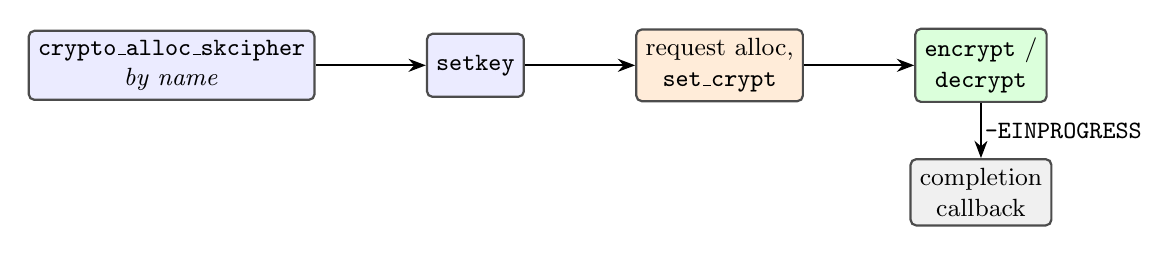
\begin{tikzpicture}[node distance=7mm and 14mm]
  \node[box,fill=blue!8] (alloc) {\code{crypto\_alloc\_skcipher}\\\emph{by name}};
  \node[box,fill=blue!8,right=of alloc] (key) {\code{setkey}};
  \node[box,fill=orange!15,right=of key] (req) {request alloc,\\\code{set\_crypt}};
  \node[box,fill=green!14,right=of req] (enc) {\code{encrypt} /\\\code{decrypt}};
  \node[box,fill=gray!12,below=of enc] (cb) {completion\\callback};
  \draw[arr] (alloc) -- (key);
  \draw[arr] (key) -- (req);
  \draw[arr] (req) -- (enc);
  \draw[arr] (enc) -- node[lbl,right]{\code{-EINPROGRESS}} (cb);
\end{tikzpicture}
\caption{Life of an operation through the crypto API.}
\end{figure}

The algorithm's \code{init} runs when a transform is created. The project's driver uses it only to set per-transform state sizes. \code{setkey} copies the key into the transform's context. The project stores the key in the context and sends it with every command, because the board keeps no per transform state for ciphers.

\section{Block cipher modes}

AES is a block cipher: it encrypts one 16 byte block under a key. A \emph{mode} says how to encrypt data longer than one block. The project provides four modes because each has a different dependency structure, and the dependency structure determines how well a request can be pipelined.

\paragraph{ECB} encrypts every block independently: $C_i = E_K(P_i)$. Identical plaintext blocks give identical ciphertext blocks, so ECB leaks structure and is not safe for real data. It is included because it is the simplest mode and a useful test: every block is independent, so every chunk is independent.

\paragraph{CBC} chains blocks: $C_i = E_K(P_i \oplus C_{i-1})$ with $C_0 = IV$. Encryption of block $i$ needs the output of block $i-1$, so it is strictly serial. Decryption is $P_i = D_K(C_i) \oplus C_{i-1}$, and every $C_{i-1}$ is part of the \emph{input}, so decryption of different blocks is independent.

\paragraph{CTR} turns the cipher into a stream cipher: $C_i = P_i \oplus E_K(\text{ctr} + i)$. The keystream blocks depend only on the counter, so every block is independent in both directions, and any length (not just a multiple of 16) is allowed.

\paragraph{GCM} is CTR for confidentiality together with GHASH for authentication (Section~\ref{sec:gcmmath}). It returns a tag that proves the data and the associated data were not modified.

\begin{table}[ht]
\centering
\begin{tabularx}{\textwidth}{lXXX}
\toprule
Mode & Encrypt & Decrypt & Length rule \\
\midrule
ECB & parallel & parallel & multiple of 16 \\
CBC & \textbf{serial} & parallel & multiple of 16 \\
CTR & parallel & parallel & any \\
GCM & parallel + one hash pass & parallel + one hash pass & any, plus a tag \\
\bottomrule
\end{tabularx}
\caption{Dependency structure of the modes.}
\end{table}

\section{Hash functions and HMAC}

A hash function maps any input to a fixed size digest: 20 bytes for SHA-1, 32 for SHA-256. It processes the input in blocks of 64 bytes, carrying a running state. That state is what makes streaming possible: a caller can add data piecemeal and ask for the digest at the end, and the crypto API's \code{init}, \code{update}, \code{final} and \code{finup} functions reflect that.

HMAC builds a keyed authentication code from a hash: $\text{HMAC}(K,m) = H((K' \oplus \text{opad}) \,\|\, H((K' \oplus \text{ipad}) \,\|\, m))$, where $K'$ is the key padded or hashed to the block size. On the board, HMAC is a normal AF\_ALG hash socket whose algorithm name is \code{hmac(sha256)} and whose key is set with the same socket option as for ciphers. The host side only forwards the key.

The crypto API also defines \code{export} and \code{import}, which save and restore the running state of a hash. This gave the project a design problem: the state lives on the board, not in the PC's memory. The solution (Section~\ref{sec:hashhost}) saves two numbers, a session id and a board id, after asking the board to \emph{clone} the session.

\section{Hardware and software providers coexisting}

A typical machine has several implementations of the same algorithm registered at once: a portable C one, an assembler one that uses processor instructions (AES-NI on x86, for example), and possibly a hardware engine. Each has a priority. When a caller asks for \code{cbc(aes)} the core picks the one with the highest priority. On the board the AM335x's OMAP crypto drivers register themselves in the same way, with higher priority than the software code, so a request for \code{cbc(aes)} on the board lands on the hardware engine without the daemon asking for it specially. The daemon's startup routine reads \code{/proc/crypto} and reports which driver is the best one for each algorithm, so the host can see what the board really uses.

\section{Synchronous and asynchronous contracts}

The asynchronous contract has a few rules that the project's code follows.

\begin{itemize}
  \item A request may return \code{-EINPROGRESS}, in which case the callback \emph{will} be called exactly once, later. It may also return \code{-EBUSY} when the driver is backlogged (the project does not use this).
  \item The request memory belongs to the caller. After the completion callback has been called, the driver must not touch the request any more. In the code this appears as a comment: \code{req (and cr) may be gone after this}, and the completion call is the last statement of the function.
  \item The driver sets \code{CRYPTO\_ALG\_ASYNC}, so callers that cannot wait for completion know not to select it. The AF\_ALG layer handles asynchronous algorithms by waiting on the caller's behalf.
  \item Completion may happen in any context. The project always completes from its workqueue, so completion is in process context.
\end{itemize}

\section{How AF\_ALG behaves in practice}

Several details of the socket interface matter in the project's code.

\begin{itemize}
  \item The \emph{bind} step names the algorithm, and for the board's own use it names a type (\code{hash}, \code{skcipher}, \code{aead}). The type decides which interface the socket exposes.
  \item The \emph{accept} step returns the operation socket. A single bound socket can accept several operation sockets, each with independent state but the same key. The daemon uses this for \code{HASH\_CLONE}: accepting again from the session socket creates a second operation that shares the key. For hashing the operation socket also inherits the running state in the implementation, which is what the clone relies on.
  \item \code{MSG\_MORE} on a send tells a hash socket that more data follows. Without it, the data is final and the digest becomes readable. The daemon uses this for \code{HASH\_UPDATE}.
  \item For ciphers the operation and IV go in control messages (\code{ALG\_SET\_OP}, \code{ALG\_SET\_IV}). The kernel carries the IV across successive sends on the same operation socket. The test helper uses this to feed large inputs in 64 KiB pieces.
  \item For GCM the associated data length and tag length are separate control and socket options (\code{ALG\_SET\_AEAD\_ASSOCLEN}, \code{ALG\_SET\_AEAD\_AUTHSIZE}).
  \item A read buffer larger than the output makes the kernel wait for more input. The demo helper reads exactly the output size for this reason.
\end{itemize}

\section{GCM mathematics}\label{sec:gcmmath}

GCM operates in the field $GF(2^{128})$ with the reduction polynomial $x^{128}+x^7+x^2+x+1$. Given the hash subkey $H = E_K(0^{128})$, GHASH of a sequence of 16 byte blocks $X_1,\ldots,X_m$ is the running value
\[
Y_0 = 0,\qquad Y_i = (Y_{i-1} \oplus X_i)\cdot H .
\]
For associated data $A$ and ciphertext $C$ the blocks are $A$ padded to a multiple of 16, then $C$ padded the same way, then one block holding the two bit lengths, $\mathrm{len}(A)\,\|\,\mathrm{len}(C)$ as two 64 bit big endian numbers. The tag is $T = \text{GHASH}_H(A,C) \oplus E_K(J_0)$, where $J_0$ is the pre-counter block, which for a 96 bit IV is $IV\,\|\,0x00000001$. The ciphertext is produced with CTR starting at $\text{inc}_{32}(J_0)$.

The only expensive step for software is the field multiplication. A simple bitwise implementation takes 128 steps per block. The daemon uses the \emph{4 bit table method}: it precomputes the sixteen multiples of $H$ for every four bit value, and then multiplies by processing the operand a nibble at a time, with a small table of reduction terms. It processes one block in 32 table lookups. The code is in \code{ghash\_init} (build the table) and \code{ghash\_mul} (use it).


\chapter{The USB gadget side}\label{ch:gadget}

\section{A computer as a USB device}

Most USB hardware is a host and a device that is a simple peripheral. A BeagleBone Black has a USB controller (the MUSB core) that can act as either. When it acts as a device, Linux on the board runs the \emph{gadget framework}. The controller is the \emph{UDC}, the USB device controller. A \emph{gadget} is a configuration of functions that the board presents.

\section{ConfigFS gadgets}

Modern kernels let user space build a gadget through \emph{configfs}, a file system of kernel objects that user space creates with \code{mkdir}. The structure used on the board is:

\begin{lstlisting}[style=shell]
/sys/kernel/config/usb_gadget/g1/          # the gadget (id 1d6b:0104)
    configs/c.1/                           # one configuration
    functions/acm.*   functions/ecm.*      # serial and ethernet
    functions/ffs.bbc                      # this project
    UDC                                    # write the controller name to start
\end{lstlisting}

Linking a function directory into a configuration adds it. Writing the name of the controller into \code{UDC} binds the gadget and makes the board appear on the USB bus. Writing an empty string unbinds it.

\section{FunctionFS}

Standard functions such as serial or network are implemented in the kernel. For a vendor specific function, Linux offers \emph{FunctionFS}. It implements the gadget side of a function in \emph{user space}. After mounting a file system of type \code{functionfs}, a program opens \code{ep0}, writes the descriptors it wants the device to present, and then opens one file per endpoint, \code{ep1}, \code{ep2} and so on. Reading an OUT endpoint file receives data from the host. Writing an IN endpoint file sends data to the host. Events such as enable and disable arrive as records on \code{ep0}.

This is the mechanism the board daemon uses. It means the board side of the project is an ordinary program, written in C, built with a cross compiler, and debuggable with ordinary tools, rather than a second kernel module.

\section{The controller on the board}

The AM335x has two USB ports, each served by a MUSB (Mentor) controller. Port 0 is wired as the mini USB connector that the PC connects to, and the Linux driver for it is the MUSB driver in dual role mode with the DSPS glue code (visible as \code{CONFIG\_USB\_MUSB\_DSPS=y} in the board kernel configuration). In device mode the controller is exposed to the gadget framework as a UDC. Its name appears in \code{/sys/class/udc/}, and the scripts read it from there.

This controller is a fixed endpoint design: it has a limited number of endpoints with fixed buffer sizes, and incoming OUT packets land in a FIFO of limited size. The consequence, documented in Chapter~\ref{ch:lessons}, is that a packet that arrives while no request is queued on its endpoint can be dropped.

\section{FunctionFS descriptors and strings}

The daemon writes a blob with three parts to \code{ep0}. A header holds a magic number, a total length and flags saying which descriptor sets follow. Then come the descriptors: a count, then the interface descriptor and the two endpoint descriptors, once for full speed and once for high speed. After the descriptor blob it writes a second blob with the strings: a count of strings and languages, the language id (0x0409, US English), and the string itself. The strings blob is required even if the function offers only one string, and the interface descriptor refers to it with \code{iInterface = 1}.

Only after both writes succeed does FunctionFS accept the gadget being bound. That is why the OpenRC service starts the daemon \emph{before} it writes the controller name into \code{UDC}.

\section{Events on endpoint zero}

After the descriptors are accepted, \code{ep0} becomes a stream of fixed size event records. The daemon cares about four.

\begin{description}
  \item[\code{FUNCTIONFS\_BIND}/\code{UNBIND}] the gadget was bound to or removed from the controller.
  \item[\code{FUNCTIONFS\_ENABLE}] the host selected the configuration. The endpoint files may now be opened, and the daemon starts its worker thread.
  \item[\code{FUNCTIONFS\_DISABLE}] the host deselected the configuration, or the cable was pulled. The daemon cancels the worker and waits for it to finish.
  \item[\code{FUNCTIONFS\_SETUP}] a control request addressed to the function. The project defines none, so the daemon answers with a stall by trying to move zero bytes the wrong way, which is the FunctionFS idiom for it.
\end{description}

\section{Bring-up order}

The order of operations on the board matters, and the OpenRC \code{start} function reproduces it exactly.

\begin{enumerate}
  \item The base gadget exists (serial and Ethernet), created by the \code{usbgadget} service, with its controller bound.
  \item Unbind the controller. This makes the board disappear from the PC for a moment.
  \item Create the function directory and link it into the configuration.
  \item Mount FunctionFS at the mount point.
  \item Start the daemon, which opens \code{ep0} and writes the descriptors.
  \item Bind the controller again. The board re-enumerates and now offers three interfaces.
  \item On the PC, the new interface matches the id table and the driver's \code{probe} runs.
\end{enumerate}

Tear down is the reverse, and the daemon must stop only after the gadget has been unbound.


% ====================================================================
\part{The \proj{} project}
% ====================================================================

\chapter{Design}\label{ch:design}

\section{Requirements}

The design started from a short list.

\begin{enumerate}
  \item Ordinary programs must be able to use the board through standard interfaces, without a custom library. This means integrating with the kernel crypto API and AF\_ALG.
  \item The driver must be a real USB driver: id table, probe, disconnect, sysfs, module parameters, clean unload.
  \item It must be correct for any input length, key size and operation order, and must be checked against a known good reference.
  \item It must survive failures. If a packet is lost the operation must still complete. If the cable is pulled, nothing may crash or hang.
  \item The board side must not require re-flashing the board. The board has no recovery path (no serial console recovery or SD card fallback was available during the work), so a bad kernel image would be expensive.
\end{enumerate}

A non-goal is speed. The measured throughput is a few megabytes per second, far below the PC's own CPU. The project demonstrates the mechanics of offload, not a performance gain.

\section{Overall structure}

Figure~\ref{fig:arch} shows the whole system.

\begin{figure}[ht]
\centering
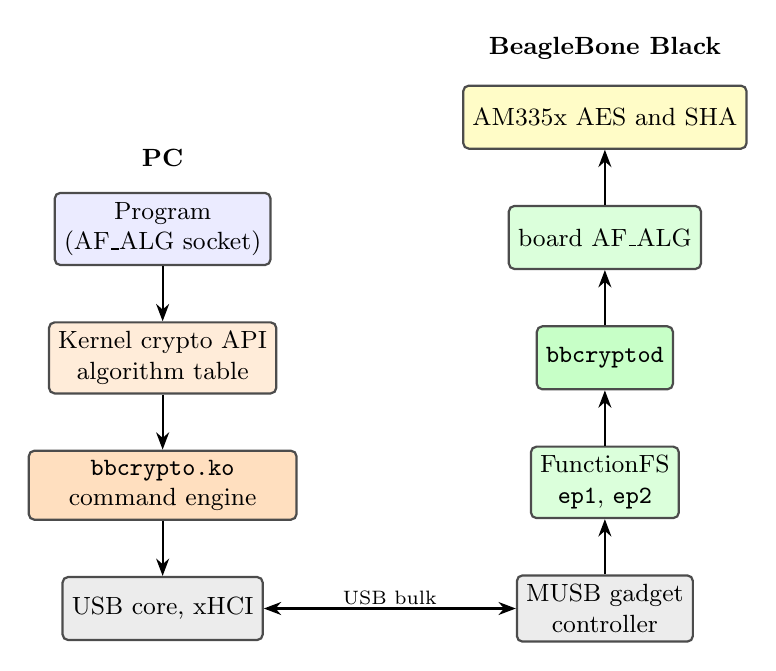
\begin{tikzpicture}[node distance=7mm and 10mm]
  \node[box,fill=blue!8] (prog) {Program\\(AF\_ALG socket)};
  \node[box,fill=orange!15,below=of prog] (crypto) {Kernel crypto API\\algorithm table};
  \node[box,fill=orange!25,below=of crypto,minimum width=3.4cm] (mod) {\code{bbcrypto.ko}\\command engine};
  \node[box,fill=gray!15,below=of mod] (usb) {USB core, xHCI};
  \node[box,fill=gray!15,right=3.2cm of usb] (musb) {MUSB gadget\\controller};
  \node[box,fill=green!14,above=of musb] (ffs) {FunctionFS\\\code{ep1}, \code{ep2}};
  \node[box,fill=green!22,above=of ffs] (dmn) {\code{bbcryptod}};
  \node[box,fill=green!14,above=of dmn] (balg) {board AF\_ALG};
  \node[box,fill=yellow!22,above=of balg] (hw) {AM335x AES and SHA};
  \draw[arr] (prog) -- (crypto);
  \draw[arr] (crypto) -- (mod);
  \draw[arr] (mod) -- (usb);
  \draw[darr] (usb) -- node[lbl,above]{USB bulk} (musb);
  \draw[arr] (musb) -- (ffs);
  \draw[arr] (ffs) -- (dmn);
  \draw[arr] (dmn) -- (balg);
  \draw[arr] (balg) -- (hw);
  \node[font=\small\bfseries,above=2mm of prog] {PC};
  \node[font=\small\bfseries,above=2mm of hw] {BeagleBone Black};
\end{tikzpicture}
\caption{System architecture. A request goes down the left side and across the USB link, and the reply returns the same way.}\label{fig:arch}
\end{figure}

\section{The central idea}

Because the board is a small, slow computer on a link that carries 512 byte packets, the design problem is to keep the link and the board busy at the same time. A simple driver would send one request, wait for the answer, and then send the next. That wastes the time the host spends preparing the next request, and the time the board spends idle. The solution is a \emph{window of commands in flight}, with tagging so replies can be matched, and a retransmission timer for lost packets. This turns a stop-and-wait protocol into a pipelined one. Figure~\ref{fig:pipe} shows the effect.

\begin{figure}[ht]
\centering
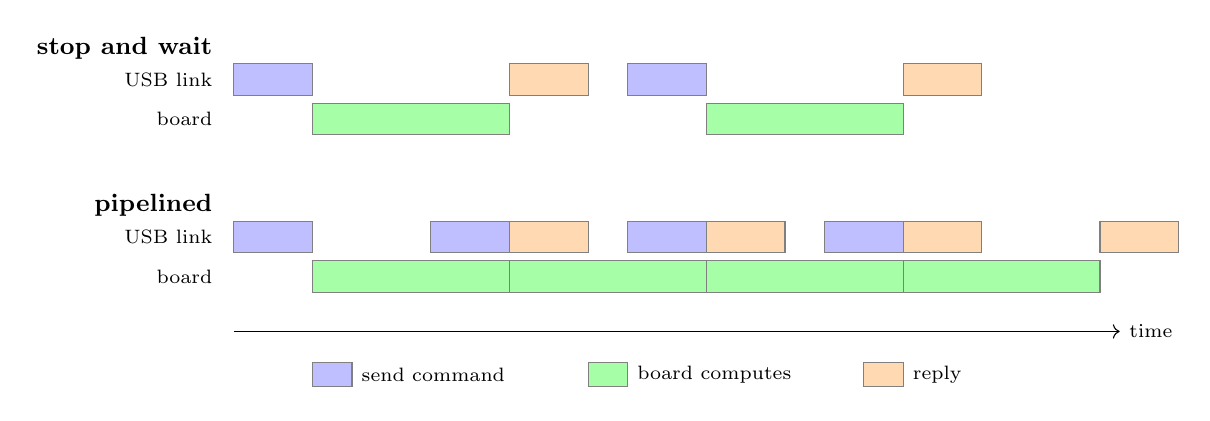
\begin{tikzpicture}[x=0.5cm,y=0.5cm]
  \tikzset{u/.style={fill=blue!25,draw=black!50},c/.style={fill=green!35,draw=black!50},r/.style={fill=orange!30,draw=black!50}}
  \node[anchor=east,font=\small\bfseries] at (-0.3,6.4) {stop and wait};
  \node[anchor=east,font=\scriptsize] at (-0.3,5.6) {USB link};
  \node[anchor=east,font=\scriptsize] at (-0.3,4.6) {board};
  \foreach \i in {0,1} {
    \draw[u] (\i*10,5.2) rectangle (\i*10+2,6.0);
    \draw[c] (\i*10+2,4.2) rectangle (\i*10+7,5.0);
    \draw[r] (\i*10+7,5.2) rectangle (\i*10+9,6.0);
  }
  \node[anchor=east,font=\small\bfseries] at (-0.3,2.4) {pipelined};
  \node[anchor=east,font=\scriptsize] at (-0.3,1.6) {USB link};
  \node[anchor=east,font=\scriptsize] at (-0.3,0.6) {board};
  \foreach \i in {0,1,2,3} {
    \draw[u] (\i*5,1.2) rectangle (\i*5+2,2.0);
    \draw[c] (\i*5+2,0.2) rectangle (\i*5+7,1.0);
    \draw[r] (\i*5+7,1.2) rectangle (\i*5+9,2.0);
  }
  \draw[->] (0,-0.8) -- (22.5,-0.8) node[right,font=\scriptsize]{time};
  \draw[u] (2,-2.2) rectangle (3,-1.6); \node[right,font=\scriptsize] at (3,-1.9) {send command};
  \draw[c] (9,-2.2) rectangle (10,-1.6); \node[right,font=\scriptsize] at (10,-1.9) {board computes};
  \draw[r] (16,-2.2) rectangle (17,-1.6); \node[right,font=\scriptsize] at (17,-1.9) {reply};
\end{tikzpicture}
\caption{Sketch of the idea (not measured). Each lane is one resource. With several commands in flight the next command is sent while the board is still computing the previous one.}\label{fig:pipe}
\end{figure}

\section{Design alternatives that were considered}

Several decisions in the design have an obvious alternative. Table~\ref{tab:alt} records what was chosen and why. The reasoning matters more than the choice, because it shows what the constraints were.

\begin{table}[ht]
\centering
\small
\begin{tabularx}{\textwidth}{p{2.9cm}p{3.4cm}X}
\toprule
Question & Chosen & Reason, and what was rejected \\
\midrule
Integration point & kernel crypto API providers & Every program can use the board unchanged. A private character device with its own ioctl interface would have needed a client library and would have been invisible to the kernel's own users. \\
Board side & user space daemon over FunctionFS & Ordinary C code, cross compiled and debugged with ordinary tools. A second kernel module on the board would have needed a kernel rebuild and re-flash, and the board had no recovery path. \\
Message framing & one request per bulk transfer & Boundaries are given by USB itself, so no length prefix scanning is needed. A byte stream over a serial style endpoint would have needed its own framing and resynchronisation. \\
Flow control & window of tagged commands & Overlaps transfer and compute. Stop and wait left both sides idle half of the time (Chapter~\ref{ch:test} measures this). \\
Loss handling & host timer plus board reply cache & Retransmission is safe because the board never executes a tag twice. Relying on USB's own retry would not cover a daemon that dropped a request it had read. \\
Ciphers & asynchronous skcipher & Matches how hardware drivers are written and lets many requests share the engine. A synchronous interface would have blocked the caller for the full round trip. \\
Hashes & synchronous shash and asynchronous ahash & The shash interface is what most in-kernel users call. The ahash interface shows the asynchronous style for hashing. Both use one engine. \\
GCM on board & assembled from CTR, ECB and software GHASH & The board kernel has no AEAD socket support. Rebuilding it was rejected as too risky. \\
Key storage & key sent with every command & The board holds no key state, so a reboot or retransmission needs no recovery logic. The cost is that keys cross the cable (Chapter~\ref{ch:security}). \\
\bottomrule
\end{tabularx}
\caption{Design decisions and the alternatives rejected.}\label{tab:alt}
\end{table}

\section{Failure model}

A design is only as good as the failures it expects. The project assumes the following can happen, and each has a mechanism that deals with it.

\begin{table}[ht]
\centering
\begin{tabularx}{\textwidth}{lXX}
\toprule
Failure & Detected by & Handled by \\
\midrule
Request packet lost on the board & no reply within one second & host resends the same tag, up to four sends \\
Reply packet lost & same timeout & the board answers the repeat from its reply cache \\
Duplicate reply arrives & no command with that tag is in flight & ignored \\
Board answers with an error & status field in the reply & error number returned to the caller \\
Garbled or unknown message & magic and length checks on both sides & dropped (the host will retry) \\
Cable pulled & URB completes with a shutdown status; disconnect is called & everything pending is completed with \code{-ENODEV} \\
No board attached & the board list is empty & new requests return \code{-ENODEV} \\
Module reloaded while the board stays up & random starting tag & stale cached replies are not matched \\
Memory allocation fails & \code{NULL} return & \code{-ENOMEM} completes the request \\
Board daemon stops answering & no reply after all retries & \code{-ETIMEDOUT} \\
\bottomrule
\end{tabularx}
\caption{Failures and their handling.}
\end{table}

\section{Who owns what}

The responsibilities of the three components are deliberately narrow.

\begin{itemize}
  \item \textbf{The module} owns the interface to the kernel (algorithms, requests, error codes), the cutting of requests into commands, windowing, matching and retransmission.
  \item \textbf{The protocol header} owns the format of every message and the limits. Neither side defines a number that the other must guess.
  \item \textbf{The daemon} owns execution: it maps an operation code to an AF\_ALG call, keeps hash sessions, remembers recent replies, and hides how the board does the work.
\end{itemize}

Because the module treats the board as a black box that executes tagged commands, the same module would work unchanged with a daemon that used a different engine, as long as it honours the protocol.

\section{Concurrency at a glance}

Figure~\ref{fig:conc} shows the threads and execution contexts in play on each side.

\begin{figure}[ht]
\centering
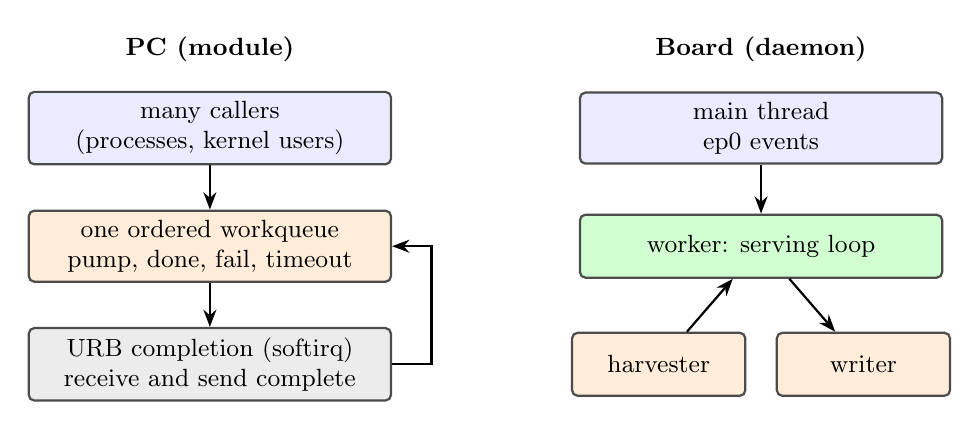
\begin{tikzpicture}[node distance=5mm and 8mm]
  \node[font=\small\bfseries] at (2.5,4.4) {PC (module)};
  \node[box,fill=blue!8,minimum width=4.6cm] (callers) at (2.5,3.4) {many callers\\(processes, kernel users)};
  \node[box,fill=orange!15,minimum width=4.6cm] (wq) at (2.5,1.9) {one ordered workqueue\\pump, done, fail, timeout};
  \node[box,fill=gray!15,minimum width=4.6cm] (irq) at (2.5,0.4) {URB completion (softirq)\\receive and send complete};
  \draw[arr] (callers) -- (wq);
  \draw[arr] (wq) -- (irq);
  \draw[arr] (irq.east) -- ++(0.5,0) |- (wq.east);

  \node[font=\small\bfseries] at (9.5,4.4) {Board (daemon)};
  \node[box,fill=blue!8,minimum width=4.6cm] (m) at (9.5,3.4) {main thread\\ep0 events};
  \node[box,fill=green!18,minimum width=4.6cm] (w) at (9.5,1.9) {worker: serving loop};
  \node[box,fill=orange!15,minimum width=2.2cm] (h) at (8.2,0.4) {harvester};
  \node[box,fill=orange!15,minimum width=2.2cm] (wt) at (10.8,0.4) {writer};
  \draw[arr] (m) -- (w);
  \draw[arr] (h) -- (w);
  \draw[arr] (w) -- (wt);
\end{tikzpicture}
\caption{Execution contexts on each side.}\label{fig:conc}
\end{figure}

On the PC, the ordered workqueue means that only one work item runs at a time per module. This removes whole classes of races between, for example, the code that emits new chunks and the code that completes a request. Callers and the URB completion handlers still run concurrently with the workqueue, and the spinlock \code{d->lock} covers them.


\chapter{The wire protocol}\label{ch:proto}

\section{Framing}

Both sides include the same header, \code{proto.h}. It defines integers as little endian and uses a conditional typedef so that the same structure compiles in the kernel (\code{\_\_le32}) and in a normal program (\code{uint32\_t}).

\begin{lstlisting}
#ifdef __KERNEL__
#include <linux/types.h>
typedef __le32 bbc_u32;
typedef __le16 bbc_u16;
#else
#include <stdint.h>
typedef uint32_t bbc_u32;
typedef uint16_t bbc_u16;
#endif
\end{lstlisting}

One request is one USB bulk transfer. It is a 32 byte header followed by the key, the initialisation vector and the data, in that order. A reply is a 24 byte header followed by an optional IV and data.

\begin{lstlisting}
struct bbc_req {            /* 32 bytes */
	bbc_u32 magic;      /* 0x43434242, "BBCC" */
	bbc_u32 tag;        /* chosen by the host, echoed in the reply */
	bbc_u16 op;
	bbc_u16 flags;
	bbc_u32 id;         /* hash session id, or assoc length */
	bbc_u32 alg;
	bbc_u32 keylen;
	bbc_u32 ivlen;
	bbc_u32 datalen;
} __attribute__((packed));

struct bbc_resp {           /* 24 bytes */
	bbc_u32 magic;
	bbc_u32 tag;
	bbc_u32 status;     /* 0 or a negative errno */
	bbc_u32 id;
	bbc_u32 ivlen;
	bbc_u32 datalen;
} __attribute__((packed));
\end{lstlisting}

Limits are compile time constants: at most 32 KiB of data, 128 bytes of key and 16 bytes of IV per request.

\section{Operations}

\begin{table}[ht]
\centering
\begin{tabularx}{\textwidth}{lX}
\toprule
Operation & Meaning \\
\midrule
\code{PING} & echo the data back, used for transport benchmarks \\
\code{INFO} & return a text description of the board's algorithm drivers \\
\code{HASH\_NEW} & start a hash session (key included for HMAC), returns an id \\
\code{HASH\_UPDATE} & feed data into a session \\
\code{HASH\_FINAL} & finish a session, return the digest, free the id \\
\code{HASH\_CLONE} & duplicate a session's state, needed for \code{export}/\code{import} \\
\code{HASH\_FREE} & discard a session \\
\code{CIPHER} & one AES operation on a chunk; reply carries the chained IV \\
\code{AEAD} & one complete GCM operation, stateless \\
\bottomrule
\end{tabularx}
\caption{Protocol operations.}
\end{table}

A one-shot flag lets a hash be computed in a single command, without creating a session, which is the fast path for small inputs.

\section{Tags, windows and retransmission}

The host numbers every command with a \emph{tag}. The tag starts at a random value for each probe and counts up. Up to \code{window} commands (4 by default, at most 8) are outstanding. The board replies in the order it processes them, and each reply carries the tag of its command, so the host finds the right command by searching its in-flight list.

Lost packets are handled on the host by a timer. A command whose reply has not arrived after 1000~ms is sent again with the \emph{same} tag. After four transmissions the command fails with \code{-ETIMEDOUT}. The board keeps its last 16 replies. When a request with a tag it has already answered arrives, it resends the cached reply instead of running the operation a second time. This matters for operations that are not idempotent. CBC encryption of a chunk with a changed chaining state would be wrong if executed twice.

The random start of the tag counter closes one subtle gap. If the module is unloaded and loaded again while the board stays up, a counter restarting from zero would collide with tags still in the board's cache, and the board would answer a new command with a stale reply. Starting from a random value makes this vanishingly unlikely.

\section{The short packet rule}\label{sec:pad}

USB ends a bulk transfer with a short packet. If a message length is an exact multiple of 512, the last packet is full and the receiver cannot tell the transfer has ended unless a zero length packet follows. The protocol avoids the zero length packet by appending one pad byte in that case. The sender adds the byte; the receiver recognises that a one byte transfer after a message whose length was a multiple of 512 is only padding and discards it. The board code has a flag (\code{expect\_pad}) for exactly this.

\section{Field by field}

The tables below spell out the headers. Offsets are in bytes from the start of the header.

\begin{table}[ht]
\centering
\begin{tabular}{rllp{7cm}}
\toprule
Offset & Size & Field & Meaning \\
\midrule
0 & 4 & \code{magic} & \code{0x43434242}, the bytes \code{42 42 43 43} on the wire \\
4 & 4 & \code{tag} & chosen by the host, echoed by the board \\
8 & 2 & \code{op} & operation code (Table~\ref{tab:ops}) \\
10 & 2 & \code{flags} & per operation flags, see below \\
12 & 4 & \code{id} & hash session id, or associated data length for \code{AEAD} \\
16 & 4 & \code{alg} & algorithm number (Table~\ref{tab:algs}) \\
20 & 4 & \code{keylen} & bytes of key that follow the header \\
24 & 4 & \code{ivlen} & bytes of IV that follow the key \\
28 & 4 & \code{datalen} & bytes of data that follow the IV \\
\bottomrule
\end{tabular}
\caption{Request header (32 bytes).}
\end{table}

\begin{table}[ht]
\centering
\begin{tabular}{rllp{7cm}}
\toprule
Offset & Size & Field & Meaning \\
\midrule
0 & 4 & \code{magic} & same constant \\
4 & 4 & \code{tag} & copy of the request's tag \\
8 & 4 & \code{status} & 0, or a negative \code{errno} as a 32 bit two's complement number \\
12 & 4 & \code{id} & new session id for \code{HASH\_NEW} and \code{HASH\_CLONE} \\
16 & 4 & \code{ivlen} & bytes of IV that follow (chained IV for ciphers) \\
20 & 4 & \code{datalen} & bytes of data that follow the IV \\
\bottomrule
\end{tabular}
\caption{Reply header (24 bytes).}
\end{table}

\begin{table}[ht]
\centering
\begin{tabular}{rl}
\toprule
Value & Operation \\
\midrule
0 & \code{PING} \\
1 & \code{HASH\_NEW} \\
2 & \code{HASH\_UPDATE} \\
3 & \code{HASH\_FINAL} \\
4 & \code{HASH\_CLONE} \\
5 & \code{HASH\_FREE} \\
6 & \code{CIPHER} \\
7 & \code{INFO} \\
8 & \code{AEAD} \\
\bottomrule
\end{tabular}
\caption{Operation codes.}\label{tab:ops}
\end{table}

\begin{table}[ht]
\centering
\begin{tabular}{rl}
\toprule
Value & Algorithm \\
\midrule
1 & SHA-1 \\
2 & SHA-256 \\
3 & HMAC-SHA-256 \\
4 & ECB-AES \\
5 & CBC-AES \\
6 & CTR-AES \\
7 & GCM-AES \\
\bottomrule
\end{tabular}
\caption{Algorithm numbers.}\label{tab:algs}
\end{table}

\paragraph{Flags.} Bit 0 means decrypt for \code{CIPHER} and \code{AEAD}. Bit 1 (\code{ONESHOT}) on \code{HASH\_NEW} asks for the digest of the attached data in the same command. For \code{AEAD}, bits 8 to 15 hold the tag length in bytes.

\section{Two messages in bytes}

\paragraph{INFO.} The first message the driver sends after probing a board is \code{INFO}, to check that the daemon is alive. With tag 42 it is a 32 byte header and nothing else:

\begin{lstlisting}[style=shell]
42 42 43 43   2a 00 00 00   07 00   00 00   00 00 00 00
magic         tag = 42      op=7    flags   id
00 00 00 00   00 00 00 00   00 00 00 00   00 00 00 00
alg           keylen        ivlen         datalen
\end{lstlisting}

The reply is a 24 byte header followed by the text that describes the board's algorithm drivers, for example \code{bbcryptod: sha1=... sha256=... cbc(aes)=cbc-aes-omap ...}. The driver stores the text and prints it when it announces the board.

\paragraph{One shot hash.} To hash the three bytes \code{abc} with SHA-256 in one command, the host sends operation 1 with flag \code{ONESHOT}, algorithm 2 and a data length of 3. The request is 35 bytes (a 32 byte header and the data). The board runs the hash and answers with a 24 byte header with status 0 and a data length of 32, followed by the 32 byte digest, in total 56 bytes. The digest of \code{abc} is the well known value

\begin{lstlisting}[style=shell]
ba7816bf 8f01cfea 414140de 5dae2223 b00361a3 96177a9c b410ff61 f20015ad
\end{lstlisting}

\paragraph{A request that needs padding.} A \code{PING} with 480 bytes of data is 32 + 480 = 512 bytes. A transfer of exactly 512 bytes would end in a full packet, so the sender adds one byte, and the board recognises and discards a following transfer of one byte.

\section{Messages for a hash session}

A hash of unknown length is a series of commands that share a session on the board (Figure~\ref{fig:hashseq}).

\begin{figure}[ht]
\centering
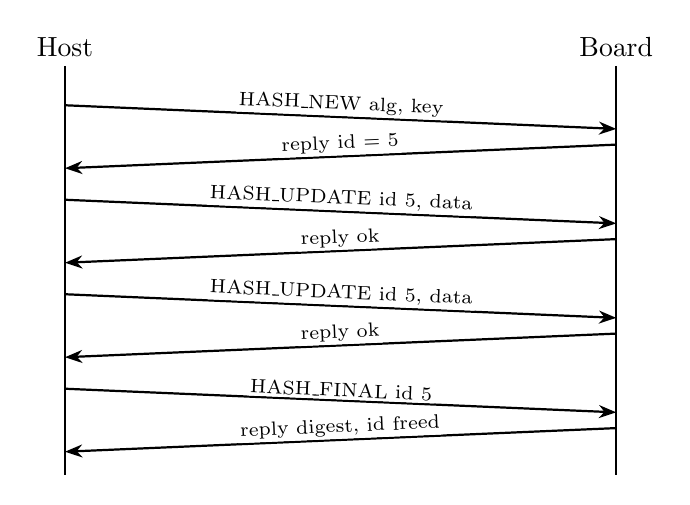
\begin{tikzpicture}[x=1cm,y=1cm]
  \draw[thick] (0,0) -- (0,-5.2); \node[above] at (0,0) {Host};
  \draw[thick] (7,0) -- (7,-5.2); \node[above] at (7,0) {Board};
  \draw[arr] (0,-0.5) -- node[lbl,above,sloped]{HASH\_NEW alg, key} (7,-0.8);
  \draw[arr] (7,-1.0) -- node[lbl,above,sloped]{reply id = 5} (0,-1.3);
  \draw[arr] (0,-1.7) -- node[lbl,above,sloped]{HASH\_UPDATE id 5, data} (7,-2.0);
  \draw[arr] (7,-2.2) -- node[lbl,above,sloped]{reply ok} (0,-2.5);
  \draw[arr] (0,-2.9) -- node[lbl,above,sloped]{HASH\_UPDATE id 5, data} (7,-3.2);
  \draw[arr] (7,-3.4) -- node[lbl,above,sloped]{reply ok} (0,-3.7);
  \draw[arr] (0,-4.1) -- node[lbl,above,sloped]{HASH\_FINAL id 5} (7,-4.4);
  \draw[arr] (7,-4.6) -- node[lbl,above,sloped]{reply digest, id freed} (0,-4.9);
\end{tikzpicture}
\caption{A streamed hash. Small inputs skip all of this with one shot hashing.}\label{fig:hashseq}
\end{figure}

The one shot flag exists because most hashes in practice are small, and a four message exchange for a 100 byte input would be dominated by round trips.

\section{Where the limits come from}

\begin{table}[ht]
\centering
\begin{tabularx}{\textwidth}{lrX}
\toprule
Limit & Value & Reason \\
\midrule
\code{BBC\_MAX\_DATA} & 32 KiB & one request must fit a bounded buffer on the board, and a bounded time on the wire \\
\code{BBC\_MAX\_KEY} & 128 bytes & AES keys are at most 32 bytes. HMAC keys can be as long as the hash block (64 bytes), and the extra headroom is cheap \\
\code{BBC\_MAX\_IV} & 16 bytes & the AES block size \\
Window & 1 to 8, default 4 & more in flight than the board's receive slots (12) and reply cache (16) can cover would break the retransmission guarantee \\
Retries & 4 sends, 1 s each & long enough for a busy daemon, short enough that a dead one is noticed \\
Reply cache & 16 entries & must exceed the window, and must exceed the writer queue (8) so a cached reply is not overwritten while it is still being sent \\
Hash sessions & 256 & each is an open socket on the board; the oldest is evicted if the table is full \\
\bottomrule
\end{tabularx}
\caption{Limits and why they have those values.}
\end{table}

\section{Status codes}

The status field in a reply is an ordinary Linux error number, negated. The driver passes it straight on to the caller, which is why a forged GCM tag reaches a user program as \code{EBADMSG} through the socket. The codes that occur are \code{-EINVAL} (bad lengths or parameters), \code{-ENOENT} (unknown hash session), \code{-EOPNOTSUPP} (unknown algorithm), \code{-ENOSYS} (unknown operation), \code{-ENOMEM}, and \code{-EBADMSG} for a failed tag check. Errors from the transport itself (\code{-ENODEV}, \code{-ETIMEDOUT}, \code{-EPROTO}, \code{-EMSGSIZE}) are generated on the host and never appear in a reply.


\chapter{The host driver}\label{ch:host}

The driver is one file of about 1,850 lines, \code{host/bbcrypto.c}. This chapter follows it from the outside in.

\section{State kept for each board}

\begin{lstlisting}
struct bbc_dev {
	struct kref ref;
	struct list_head node;       /* in the global list of boards */
	u32 devid;
	struct usb_device *udev;
	struct usb_interface *intf;
	unsigned int pipe_out, pipe_in;

	spinlock_t lock;
	bool dead;
	u32 tag;
	struct list_head queue;      /* waiting for a window slot */
	struct list_head inflight;   /* sent, awaiting a reply */
	struct list_head donelist;   /* finished, waiting for ->done() */
	struct list_head active;     /* cipher requests with chunks left */
	unsigned int n_queued, n_inflight, max_inflight;

	struct work_struct pump_work, done_work, fail_work;
	struct delayed_work to_work;
	struct usb_anchor anchor;
	struct urb *rx_urb;
	...
};
\end{lstlisting}

The structure reads like a diagram of the engine. A command moves from \code{queue} to \code{inflight} to \code{donelist}. The three work items correspond to three jobs that cannot be done in interrupt context: \code{pump\_work} starts new commands, \code{done\_work} runs completion callbacks, and \code{fail\_work} cleans up after a disconnect. The delayed work \code{to\_work} is the retransmission timer.

\section{The command engine}

A \code{struct bbc\_cmd} represents one command. It owns its URB, its output buffer (the request as it goes on the wire), its reply buffer, its tag, a retry count, and a completion callback. It has a reference count because several parties hold it: the engine, the URB currently in flight, and sometimes a thread waiting synchronously.

The life of a command (Figure~\ref{fig:cmd}):

\begin{figure}[ht]
\centering
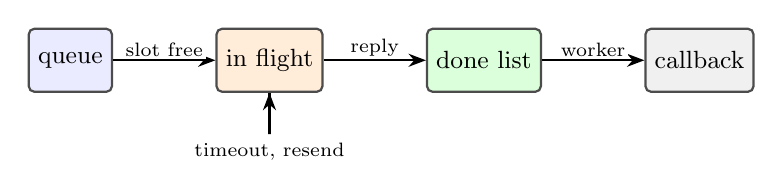
\begin{tikzpicture}[node distance=9mm and 13mm]
  \node[box,fill=blue!8] (q) {queue};
  \node[box,fill=orange!15,right=of q] (i) {in flight};
  \node[box,fill=green!14,right=of i] (d) {done list};
  \node[box,fill=gray!12,right=of d] (c) {callback};
  \draw[arr] (q) -- node[lbl,above]{slot free} (i);
  \draw[arr] (i) -- node[lbl,above]{reply} (d);
  \draw[arr] (d) -- node[lbl,above]{worker} (c);
  \draw[arr,rounded corners=3pt] (i) -- ++(0,-1.0) -| node[lbl,pos=0.25,below]{timeout, resend} (i);
\end{tikzpicture}
\caption{States of a command in the engine.}\label{fig:cmd}
\end{figure}

\begin{enumerate}
  \item A caller builds a command and submits it. It lands on \code{queue}.
  \item \code{bbc\_send\_queued} moves commands to \code{inflight} while fewer than \code{window} are outstanding. It records the send time and arms the timer. It sends the command's URB.
  \item The always-posted receive URB completes with a reply. \code{bbc\_rx\_complete} searches \code{inflight} for the tag, copies the reply into the command's buffer, and moves the command to \code{donelist}.
  \item \code{done\_work} runs the callbacks from process context, then starts more commands.
\end{enumerate}

The receive path never lets the board's reply find no URB waiting. One receive URB is always posted. When it completes, the handler processes it and resubmits it at once. This is the one place the driver posts an URB from interrupt context, and the reason it uses \code{GFP\_ATOMIC} there.

\begin{lstlisting}
resubmit:
	if (READ_ONCE(d->dead))
		return;
	usb_anchor_urb(u, &d->anchor);
	ret = usb_submit_urb(u, GFP_ATOMIC);
\end{lstlisting}

If a reply matches no command, the handler ignores it. That happens when the board replays a cached reply for a command that already finished, and it is the normal sign that a retransmission and the original answer crossed.

\section{Timeouts and retries}

\code{bbc\_to\_work} runs every 100~ms while anything is in flight. It looks for commands whose last send is older than one second and whose output URB has already finished (\code{waiting} is set). It increments the retry counter, marks the command for resending, and sends it again outside the lock. After four attempts the command fails. Statistics count the retries, and in the final test run there were none.

\section{Ciphers}

A cipher request may be megabytes long, but a protocol command carries at most 32 KiB. The driver cuts a request into chunks of \code{chunk} bytes (16 KiB by default, a multiple of 16, adjustable at run time). How the chunks are chained depends on the mode.

\begin{table}[ht]
\centering
\begin{tabularx}{\textwidth}{lXl}
\toprule
Mode & Dependency between chunks & Pipelined \\
\midrule
ECB & none & yes \\
CTR & none, once the counter for each chunk is computed in advance & yes \\
CBC decrypt & chaining input is the previous \emph{ciphertext} block, known up front & yes \\
CBC encrypt & chaining input is the previous \emph{output}, known only after the board replies & no, one at a time \\
\bottomrule
\end{tabularx}
\caption{Chunking rules.}
\end{table}

For CTR the driver advances the counter by the number of blocks in each chunk with a big number addition (\code{bbc\_ctr\_add}). For CBC decryption it copies the last ciphertext block of a chunk into the IV for the next chunk before the chunk is even sent. For CBC encryption the board returns the new chaining value in the reply's IV field, and the driver uses it for the next chunk. That is an inherent serial dependency, and it is why CBC encryption cannot overlap its chunks.

The entry point returns \code{-EINPROGRESS}:

\begin{lstlisting}
	list_add_tail(&cr->node, &d->active);
	spin_unlock_irqrestore(&d->lock, fl);
	bbc_kick(d, &d->pump_work);
	return -EINPROGRESS;
\end{lstlisting}

The request is placed on the \code{active} list and the pump work emits chunks as window slots become free. When all chunks have finished, the last one completes the original request.

\section{Hashes}

Hashing keeps the synchronous \code{shash} interface but still runs through the engine, so threads that hash at the same time pipeline their commands. A hash descriptor remembers the board and the session id. The first \code{update} creates a session on the board with \code{HASH\_NEW}, later updates add data, and \code{final} fetches the digest. A hash session lives on one board, so the descriptor stores the device id and later calls use \code{bbc\_get\_id} to find the same board again.

An asynchronous variant (\code{ahash}) registers the same algorithms under the names \code{sha1-async-bbcrypto}, \code{sha256-async-bbcrypto} and \code{hmac-sha256-async-bbcrypto}. It steps through the same sequence from callbacks.

\section{GCM}

GCM is registered as an \code{aead} algorithm. One request is one \code{AEAD} command: the data field holds the associated data followed by the text, plus the tag when decrypting. The associated data length goes in the request's \code{id} field and the tag length in the upper byte of \code{flags}. The reply holds the result. A forged tag comes back as status \code{-EBADMSG}, which the driver passes up to the caller unchanged. A request is limited to 32 KiB of associated data and text together.

\section{Several boards}

More than one board can be attached. A global list holds them. New cipher requests are spread round robin by \code{bbc\_get}, which advances a pointer through the list and takes a reference on the chosen board. Hash sessions stay on the board that created them.

\section{Probe and disconnect}\label{sec:probe}

The probe function does the following, in this order:

\begin{enumerate}
  \item Find the bulk IN and OUT endpoints with \code{usb\_find\_common\_endpoints}.
  \item Allocate the per board structure, initialise the lists, locks and work items, choose a random starting tag.
  \item Allocate the receive buffer and URB, and \emph{post the receive URB}.
  \item Send an \code{INFO} command and wait. If the daemon does not answer, the probe fails. This proves the whole path works before anything is registered.
  \item Create the sysfs files \code{stats} and \code{ping}.
  \item Add the board to the global list. If this is the first board, register the crypto algorithms.
\end{enumerate}

Each step has a label in the error path that undoes the steps before it, the standard kernel \code{goto} cleanup pattern.

Disconnect has to be careful in the other direction. It first removes the board from the list so no new request picks it, then sets the \code{dead} flag under the lock, kills all anchored URBs, cancels the timer, runs the failure work (which completes every pending request with an error), removes the sysfs files and drops its reference.

One design decision deserves explanation. \emph{The algorithms stay registered after the last board disconnects.} The crypto core warns when an algorithm is unregistered while a transform for it still exists, and a program can hold an open AF\_ALG socket for as long as it likes. So the algorithms are only unregistered at module unload, which the kernel will not allow while a transform holds a reference to the module. While no board is attached, requests fail with \code{-ENODEV}.

\section{Observability}

Two sysfs files are provided on each board's interface directory.

\paragraph{\code{stats}} reports the number of requests, bytes, errors and retries, the average latency in microseconds, the current and highest number of commands in flight, and the board's description string. The test suite and several demos read it to prove that work really reached the board.

\paragraph{\code{ping}} runs a transport benchmark using the \code{PING} command, which echoes data without computing anything. It measures the USB path alone, separately from the cryptography.

\section{Building a command}

Every operation starts in \code{bbc\_cmd\_new}. It allocates five things: the command structure, a buffer for the outgoing message, a buffer for the reply, an URB, and takes a reference on the board. If any allocation fails, everything allocated so far is freed and \code{NULL} is returned, so callers have a single failure case to check.

The function then writes the header in little endian with \code{cpu\_to\_le32} and \code{cpu\_to\_le16}, which are no-ops on a little endian PC and a byte swap on a big endian one, followed by the key and IV. It does \emph{not} copy the data. It returns a pointer to where the data belongs, and the caller copies into it from the request's scatterlist. This avoids an intermediate buffer. If the total message length is a multiple of 512, the function appends the pad byte.

A command receives its tag only when it is submitted (\code{bbc\_cmd\_submit}), under the board's lock: \code{c->tag = ++d->tag}. Doing it under the lock makes tags unique and increasing per board even when many threads submit at the same time, and means that a command built but never submitted never uses a tag.

\section{The engine in motion}

Follow one command through the code.

\begin{enumerate}
  \item \code{bbc\_cmd\_submit} stores the callback, takes a timestamp for the latency statistic, assigns the tag, puts the command on \code{queue}, and calls \code{bbc\_kick} for the pump work. If the board is already dead it completes the command with \code{-ENODEV} instead.
  \item \code{bbc\_pump\_work} first lets cipher requests emit more chunks (\code{bbc\_emit\_chunks}), then sends queued commands (\code{bbc\_send\_queued}).
  \item \code{bbc\_send\_queued} loops. Under the lock it checks the window: if the board is dead, or \code{n\_inflight} has reached the window, or the queue is empty, it stops. Otherwise it moves the first command to \code{inflight}, sets its state, resets its attempts to one, records the send time, updates the high-water mark, takes a reference for the URB and arms the timer. It then leaves the lock and submits the URB.
  \item The output URB completes in \code{bbc\_out\_complete}. If it failed, the command is finished with that status. If it succeeded, the command is marked \code{waiting}, which tells the timer that the reply clock is now running. The URB's reference is dropped.
  \item The reply arrives on the always-posted receive URB, and \code{bbc\_rx\_complete} finds the command by tag.
  \item The handler checks the reply is long enough for what its header claims and that it fits in the command's reply buffer, then copies it in and calls \code{bbc\_finish\_locked}, which moves the command to \code{donelist}.
  \item \code{bbc\_done\_work} runs the callbacks, updates the counters, and finally calls \code{bbc\_emit\_chunks} and \code{bbc\_send\_queued} again because slots have been freed.
\end{enumerate}

Notice that step 3 sets the timer arm \emph{inside} the lock, with a comment that says why: so that a disconnect, which sets \code{dead} under the same lock, wins the race. Without that, a retransmission timer could be armed on a board that is already being torn down.

\section{Why the receive handler copies}

The handler copies the whole reply into the command's own buffer rather than handing over a pointer to the shared receive buffer. The shared buffer is reused for the next reply as soon as the URB is resubmitted, which happens immediately. A copy of at most 32 KiB per reply is cheap, and it means every command owns its result, so the rest of the driver never has to worry about the buffer being overwritten under it.

\section{Hash sessions on the host}\label{sec:hashhost}

The synchronous hash functions in \code{bbc\_hash\_*} keep a small per-request structure:

\begin{lstlisting}
struct bbc_hash_desc {   /* per request; id 0 = no board session yet */
	u32 id;
	u32 devid;       /* the board that holds the session */
};
\end{lstlisting}

\paragraph{Lazy session creation.} \code{init} does nothing on the board. It only zeroes the structure. The session is created on the first \code{update}. This means that a hash which is started and never used costs nothing, and that the common case, a single \code{digest} call, never creates a session at all.

\paragraph{One shot.} \code{final} with no existing session and at most 32 KiB of data uses the \code{ONESHOT} command: one round trip, key and data in, digest out.

\paragraph{Streaming.} \code{update} cuts data into pieces of at most 32 KiB and sends one \code{HASH\_UPDATE} each, in order, waiting for each reply (the calls are synchronous). \code{final} sends \code{HASH\_FINAL} and clears the session id, because the board frees the session on its own.

\paragraph{Export and import.} The crypto API may ask a hash to save its state and later restore it, possibly twice. The state is on the board, so \code{export} asks the board to clone the session and writes two numbers, the \emph{new} session id and the board's id, into the saved state, which is eight bytes in total (\code{statesize = 2 * sizeof(u32)}). \code{import} reads them back. The saved session stays on the board, which means an exported state that is never imported is leaked on the board until the daemon's table evicts it. The code comment in the daemon says so.

\paragraph{Why each call is a synchronous round trip.} The hash interface here is \code{shash}, which has no completion callback. So each \code{bbc\_xfer} sleeps until its reply arrives. Parallelism comes from many callers, each blocked in its own thread, with their commands interleaved in the window. This is the setting demo~5 uses: 64 threads hashing at the same time.

\section{The asynchronous hash state machine}

The \code{ahash} implementation cannot sleep, so each step is a separate command whose completion starts the next. A request carries a stage (\code{AH\_NEW}, \code{AH\_UPD}, \code{AH\_FIN} or \code{AH\_ONE}) and an offset into the data (Figure~\ref{fig:ahstate}).

\begin{figure}[ht]
\centering
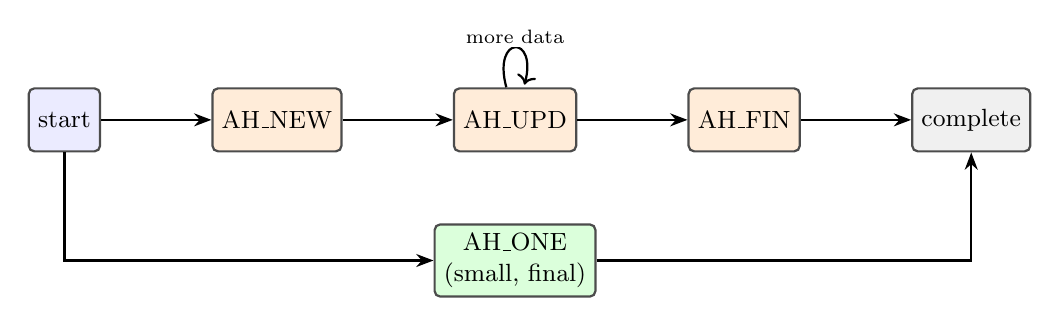
\begin{tikzpicture}[node distance=9mm and 14mm]
  \node[box,fill=blue!8] (s) {start};
  \node[box,fill=orange!15,right=of s] (new) {AH\_NEW};
  \node[box,fill=orange!15,right=of new] (upd) {AH\_UPD};
  \node[box,fill=orange!15,right=of upd] (fin) {AH\_FIN};
  \node[box,fill=green!14,below=of upd] (one) {AH\_ONE\\(small, final)};
  \node[box,fill=gray!12,right=of fin] (done) {complete};
  \draw[arr] (s) -- (new);
  \draw[arr] (new) -- (upd);
  \draw[arr] (upd) edge[loop above] node[lbl,above]{more data} (upd);
  \draw[arr] (upd) -- (fin);
  \draw[arr] (fin) -- (done);
  \draw[arr] (s) |- (one);
  \draw[arr] (one) -| (done);
\end{tikzpicture}
\caption{Stages of an asynchronous hash request.}\label{fig:ahstate}
\end{figure}

\code{bbc\_ah\_step} decides which command to send next from the state (does a session exist, is there data left, is this the final call). \code{bbc\_ah\_done} reads the reply and either calls \code{bbc\_ah\_step} again or completes the request. Because the step function is called from a completion callback, and callbacks run on the workqueue, no recursion builds up on the stack.

The state machine also handles an edge case: an \code{update} of zero bytes with no session, which the crypto layer can issue, finishes at once without touching the board.

\section{Cipher requests: a worked example}

Take an ECB request of 100000 bytes with the default chunk of 16384 and window of 4.

\begin{table}[ht]
\centering
\begin{tabular}{rrrl}
\toprule
Chunk & Offset & Length & Message size on the wire \\
\midrule
1 & 0 & 16384 & $32 + 32 + 16384 = 16448$ \\
2 & 16384 & 16384 & 16448 \\
3 & 32768 & 16384 & 16448 \\
4 & 49152 & 16384 & 16448 \\
5 & 65536 & 16384 & 16448 \\
6 & 81920 & 16384 & 16448 \\
7 & 98304 & 1696 & $32 + 32 + 1696 = 1760$ \\
\bottomrule
\end{tabular}
\caption{Chunks of a 100000 byte ECB request with a 256 bit key. ECB has no IV, so only header and key precede the data.}
\end{table}

Seven commands, with up to four on the wire at once. When one of the first four completes, the engine emits chunk 5 into the freed slot, and so on. For CBC encryption the same request runs the seven chunks \emph{one at a time}, because each chunk needs the chaining value from the reply of the one before it. The field \code{serial} in the request structure is set for exactly that case, and the emit loop's rule \code{it->inflight >= (it->serial ? 1 : win())} enforces it.

\paragraph{Fairness.} If several cipher requests are active, \code{bbc\_emit\_chunks} takes a chunk from the first request that can emit one and then moves that request to the end of the list. The requests thus take turns, and a long request cannot starve a short one that arrived later.

\paragraph{Completion.} Each chunk's callback copies its result into the destination scatterlist at the chunk's offset, decreases the in-flight count, and calls \code{bbc\_creq\_progress}. That function does nothing until nothing is in flight and no chunk is left to emit. Then it removes the request from the active list, writes the final IV back to the request (callers of CBC and CTR expect the IV to be updated), and calls \code{skcipher\_request\_complete}. If any chunk failed, the first error is remembered, no more chunks are emitted, and the error is returned once the chunks already in flight have finished.

\section{Counter arithmetic}

The CTR counter is a 128 bit big endian number. Advancing it by the number of blocks in a chunk is a multiword addition with carry, done byte by byte from the least significant end in \code{bbc\_ctr\_add}. The daemon has a twin of this function (\code{ctr\_add}) so that it can return the incremented counter to the host after a CTR chunk. Both sides agree on the arithmetic, and a test with a 1 MiB CTR request checks that chunk boundaries do not break the stream.

\section{The synchronous helper}

\code{bbc\_xfer} wraps a command in a completion. It builds the command, takes an extra reference for itself, submits with a callback that completes the completion, and sleeps. When woken it first looks at the transport status, then at the board's status in the reply, and then copies the optional IV and data out to the caller's buffers, checking that they fit. Probe uses it for \code{INFO}, and the hash functions use it for everything.

\section{AEAD mapping}

\code{bbc\_aead\_crypt} maps one crypto request to one command. The kernel passes the associated data and the text in the same source scatterlist, and the project's command carries them in one data field, so a single \code{sg\_pcopy\_to\_buffer} of \code{assoclen + cryptlen} bytes is all it needs. The associated data length goes into the header's \code{id} field. On decryption the data field also holds the tag at the end, and the request is rejected beforehand if it is shorter than the tag. The result is copied back with one \code{sg\_pcopy\_from\_buffer}. The 32 KiB limit applies to the sum of the associated data, the text and the tag.

\section{The ping benchmark}

\code{ping\_store} parses two numbers, a size and a count, from what was written to the file. It sends \code{PING} commands through the normal engine, so the window applies, and measures the time with \code{ktime\_get}. It primes the pipeline with twice the window of commands, and each completion callback submits the next one until the count is reached. A guard (an extra pending count) prevents the completion firing before the priming loop is done. The result is a formatted line stored in the board structure and shown when the file is read, with the total time, the time per command and the throughput in KB/s. Section~\ref{sec:transport} shows what it measured.


\chapter{The board side}\label{ch:board}

\section{The platform}

The board runs a Linux kernel configured for the AM335x. The configuration (kept in \code{board/kernel.config}) has the pieces the project needs: the MUSB controller in dual-role mode, configfs gadgets with the FunctionFS function, the user space crypto interfaces for hashing and symmetric ciphers, and the OMAP crypto drivers for AES and SHA (\code{CRYPTO\_DEV\_OMAP\_AES}, \code{CRYPTO\_DEV\_OMAP\_SHAM}). The userland is Alpine Linux with OpenRC and musl libc.

The kernel was built without the AEAD interface for AF\_ALG (\code{CRYPTO\_USER\_API\_AEAD} is off). That has a consequence handled in Section~\ref{sec:gcmboard}.

\section{Setting up the gadget}

Two OpenRC services start the board side. \code{usbgadget} creates the base gadget with serial and Ethernet functions, which are the board's management path. \code{bbcrypto} adds the FunctionFS function to it, starts the daemon, and rebinds the controller. The relevant steps of its \code{start} function are:

\begin{lstlisting}[style=shell]
unbind                                   # write "" to UDC
mountpoint -q $MNT && umount $MNT
mkdir $F                                 # functions/ffs.bbc
ln -s $F $G/configs/c.1/ffs.bbc          # add it to the configuration
mkdir -p $MNT
mount -t functionfs bbc $MNT
start-stop-daemon --start --background ... bbcryptod $MNT
sleep 1
echo "$UDC" > $G/UDC                     # bind: the board re-enumerates
\end{lstlisting}

Two details came from experience. The daemon has to be running \emph{before} the gadget is bound, because FunctionFS needs its descriptors before the host sees the device. And the daemon must never be killed while the gadget is bound: doing so hung the board's kernel twice. The scripts therefore always unbind first. If binding fails, the script restores the original serial and Ethernet gadget so the board stays reachable.

\section{The descriptors}

The daemon builds its descriptors in the program and writes them to \code{ep0}. The interface has class 0xff (vendor specific), subclass 0x5c, protocol 1, and two bulk endpoints, OUT on 1 and IN on 2. The full speed descriptor uses a 64 byte maximum packet size and the high speed one uses 512. The interface string is \code{bbcrypto accel}.

\section{Daemon structure}

The daemon is organised as threads around one serving loop (Figure~\ref{fig:daemon}).

\begin{figure}[ht]
\centering
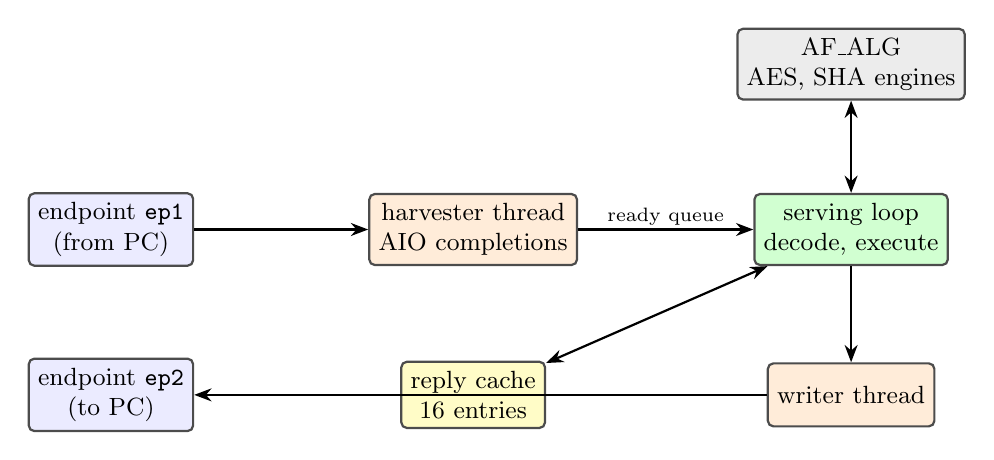
\begin{tikzpicture}
  \node[box,fill=blue!8] (ep1) at (0,0) {endpoint \code{ep1}\\(from PC)};
  \node[box,fill=orange!15] (rx) at (4.6,0) {harvester thread\\AIO completions};
  \node[box,fill=green!18] (srv) at (9.4,0) {serving loop\\decode, execute};
  \node[box,fill=gray!15] (alg) at (9.4,2.1) {AF\_ALG\\AES, SHA engines};
  \node[box,fill=yellow!22] (cache) at (4.6,-2.1) {reply cache\\16 entries};
  \node[box,fill=orange!15] (wr) at (9.4,-2.1) {writer thread};
  \node[box,fill=blue!8] (ep2) at (0,-2.1) {endpoint \code{ep2}\\(to PC)};
  \draw[arr] (ep1) -- (rx);
  \draw[arr] (rx) -- node[lbl,above]{ready queue} (srv);
  \draw[darr] (srv) -- (alg);
  \draw[arr] (srv) -- (wr);
  \draw[arr] (wr) -- (ep2);
  \draw[darr] (srv) -- (cache);
\end{tikzpicture}
\caption{Threads of the board daemon.}\label{fig:daemon}
\end{figure}

\paragraph{Reading with asynchronous I/O.} The daemon does not simply call \code{read} in a loop. On the AM335x gadget controller a packet that arrives while no read is queued on the endpoint can be lost. The first 512 byte packet of an OUT transfer disappears. A loop that calls \code{read}, handles the data and calls \code{read} again always leaves a short gap, and when the host pipelines several requests that gap is hit constantly. The daemon therefore uses the kernel's AIO interface to keep twelve read requests (\code{NSLOT}) queued on the endpoint at all times. The harvester thread collects completions, reassembles a request that arrived in several pieces, discards pad bytes, and puts complete requests on a ready queue. A request buffer is only taken out of the queue while it is being served, and then re-submitted.

\paragraph{The serving loop.} It takes a request from the ready queue, checks the magic and lengths, and looks the tag up in the reply cache. A cached tag means a retry, so the cached reply is re-sent and nothing is executed. Otherwise the operation code selects a handler. The reply is built in a cache slot (so it can be replayed later), and handed to the writer.

\paragraph{The writer thread.} Sending replies on a separate thread lets the serving loop begin the next request while the previous reply goes over USB. The extra thread handoff costs a little for tiny requests, which is a known trade off.

\section{Executing operations}

The daemon uses the board's crypto through AF\_ALG, the same interface a PC program uses. For a cipher it opens a socket bound to the algorithm \code{ecb(aes)}, \code{cbc(aes)} or \code{ctr(aes)}, sets the key, sends the data with an operation and IV as control messages, and reads the result. On the AM335x those names resolve to the OMAP drivers such as \code{cbc-aes-omap}.

After a cipher operation the daemon computes the chaining value for the next chunk and returns it in the reply: for CBC the last ciphertext block, and for CTR the incremented counter.

Hash sessions are held in a table of 256 slots, each keeping the AF\_ALG operation socket open between updates. \code{HASH\_CLONE} duplicates a session by accepting a new socket from the existing one.

\section{GCM on the board}\label{sec:gcmboard}

Because the board kernel has no AEAD interface for AF\_ALG, the AM335x GCM driver cannot be used from user space. Rebuilding and re-flashing the board kernel was rejected, because the board had no recovery path. Instead the daemon assembles GCM from parts, using the hardware for the part that costs time.

GCM encrypts with counter mode and authenticates with GHASH, a polynomial hash in the field $GF(2^{128})$. The daemon computes:

\begin{align*}
H &= E_K(0^{128}) &&\text{(hash subkey, one ECB block)}\\
J_0 &= IV \,\|\, 0^{31}1 &&\text{(for a 96 bit IV)}\\
\text{keystream} &= E_K(J_0),\, E_K(J_0+1),\ldots &&\text{(one CTR run)}\\
C &= P \oplus \text{keystream}_{1..}\\
T &= \text{GHASH}_H(A, C) \oplus E_K(J_0)
\end{align*}

The trick is that one CTR operation over $16$ zero bytes followed by the text yields both $E_K(J_0)$ (the first keystream block, used as the tag mask) and the ciphertext keystream (the rest). So AES work stays on the hardware engine, and only GHASH is computed in software, using a 4 bit table method for the multiplication. Tags up to 16 bytes (the lengths the kernel's GCM check accepts) and any associated data length are supported, and the tag comparison on decrypt runs over all bytes without an early exit, so its time does not reveal where a forged tag first differs. A mismatch returns \code{-EBADMSG}. The code notes that if the board kernel is rebuilt with AEAD support, this function can be replaced by a single AF\_ALG call.

\section{Handling the USB side}

The main thread reads events from \code{ep0}. On \code{ENABLE} (the host selected the configuration) it starts a worker thread that opens \code{ep1} and \code{ep2} and runs the serving loop. On \code{DISABLE} it cancels the worker. Control requests that arrive for the interface are answered with a stall, since none are defined.

\section{Startup and the information string}

When the daemon starts it first builds its description. \code{build\_info} reads \code{/proc/crypto}, a text file with blocks of lines for each registered algorithm, and for each of the seven algorithms the project cares about it finds the driver with the highest priority. It writes a line such as \code{bbcryptod: sha256=omap-sha256 cbc(aes)=cbc-aes-omap \ldots} into a 256 byte buffer. This string is returned by \code{INFO} and logged by the host driver at probe time, so an operator can see on the PC which engine will really do the work.

The daemon then opens \code{ep0}, writes the descriptors and strings, and enters the event loop described in Chapter~\ref{ch:board}.

\section{AF\_ALG on the board}

All cryptography on the board goes through one helper, \code{alg\_open}. It creates a socket, binds it to a type and a name, sets the key, optionally sets the tag size, and calls \code{accept} to get the operation socket. It returns the operation socket and, through a pointer, the bound socket. The bound socket is usually closed straight away, since the operation socket keeps the transform alive. Error handling closes whatever was opened and returns a negative \code{errno}, so callers can put the number straight into the reply status.

For ciphers each request opens a fresh transform. That costs a few system calls but avoids any cache of keys on the board. Key material therefore lives on the board only for the length of one request.

\section{Hash sessions}

A hash session is an open operation socket. The daemon keeps 256 slots in a table, each holding the file descriptor and a sequence number. Id 0 is invalid. \code{sess\_add} fills the first free slot and, when the table is full, evicts the one with the lowest sequence number, which is the least recently used. \code{sess\_fd} refreshes the sequence number on each use. This eviction exists so that sessions leaked by a crashed or unplugged host cannot fill the table forever.

\begin{table}[ht]
\centering
\begin{tabularx}{\textwidth}{lX}
\toprule
Operation & What the daemon does \\
\midrule
\code{HASH\_NEW} & open a hash socket with the key (for HMAC); with \code{ONESHOT}, send the data without \code{MSG\_MORE} and read the digest, close; otherwise store the socket and return its slot as the id \\
\code{HASH\_UPDATE} & \code{send} the data with \code{MSG\_MORE} on the session's socket \\
\code{HASH\_FINAL} & \code{send} any remaining data without \code{MSG\_MORE}, then read the digest (up to 64 bytes, the largest digest), free the slot \\
\code{HASH\_CLONE} & \code{accept} again on the session socket, which duplicates the state, store the new socket and return its slot \\
\code{HASH\_FREE} & close the socket and free the slot \\
\bottomrule
\end{tabularx}
\caption{Hash operations on the board.}
\end{table}

\section{Cipher handling details}

\code{do\_cipher} builds a control message with the operation (encrypt or decrypt) and, for modes with an IV, a second control message with the IV. It sends the data with \code{sendmsg} and reads exactly as many bytes back as it sent. After success it computes the IV to return. For CBC that is the last block of the \emph{ciphertext}, which is the output when encrypting and the input when decrypting; for CTR it is the counter advanced by the number of blocks. For ECB nothing is returned. The host uses these values as described in Chapter~\ref{ch:host}.

\section{The receive state machine}

The harvester thread is the most intricate code in the daemon, because it must cope with three things that the USB layer can do to a message: split it into several reads, append a pad byte, or lose its first packet.

\begin{enumerate}
  \item It waits for completions of the queued reads with \code{io\_getevents} and a 100 ms timeout so that it notices a request to quit.
  \item For each completed read it first checks whether the previous message ended with a multiple of 512 bytes and a pad byte is therefore expected. A read of exactly one byte at that point is that pad: it is discarded and its buffer is queued again.
  \item If a message is being assembled and the new read does \emph{not} start with a request header magic, it is the next piece of that message: it is appended to the assembly buffer. When enough bytes have arrived, the message is pushed to the ready queue.
  \item If a message is being assembled and the new read \emph{does} start with a header, the rest of the old message was lost. The old buffer is discarded and queued again, and the new read starts a fresh message. The host's retry will deliver the lost one again.
  \item A read that starts with a header, and is long enough to contain the whole message according to the lengths in its header, goes straight to the ready queue. A shorter one starts an assembly.
  \item Anything else (no magic, impossible lengths) is logged as bad data and dropped.
\end{enumerate}

Before any buffer is used, the lengths in the header are checked against the maximum message size. A header cannot make the daemon read beyond its buffer.

\section{Invariants between the queues}

Three numbers have to be in the right order for the retransmission guarantee to hold.

\[
\text{window (at most 8)} \;<\; \text{read slots (12)} \quad\text{and}\quad \text{writer queue (8)} \;<\; \text{reply cache (16)}
\]

The first inequality says the daemon always has a read queued for the next request even with a full window in flight. The second says that a reply entry is never overwritten for a newer reply while the writer thread is still sending it: the writer can be at most eight replies behind, and the cache keeps sixteen. The daemon's comments state these rules, and the window limit of 8 in the host driver is chosen to respect them.

\section{Reply path}

The reply is assembled directly into a cache slot, so no second copy is needed to keep it for replay. The slot is picked round robin. Its length is set to zero while it is being filled, so a concurrent lookup of the tag does not find a half built entry. When the reply is complete, its tag and length are set, and it is placed on the writer's queue. The queue is bounded by a counting semaphore, so if the writer falls behind, the serving loop waits instead of overwriting.

If a write to the endpoint fails (the host disappeared), the writer sets a flag and wakes the serving loop through a sentinel on the ready queue. The loop then ends, \code{rx\_stop} cancels the writer and the harvester, destroys the AIO context, and the worker closes the endpoint files. The main thread is notified by the \code{DISABLE} event and is ready to start a new worker on the next \code{ENABLE}.

\section{GHASH implementation notes}

\code{ghash\_init} builds a table of sixteen entries, one for each four bit value, holding that value times $H$. It computes the entries for 8, 4, 2 and 1 by repeated halving with reduction (the field's ``multiply by $x$'' step), and fills the rest by xor of those, because multiplication in the field is linear. \code{ghash\_mul} then walks the 16 bytes of the operand from the end, two nibbles per byte, shifting the accumulator right by four bits each step and folding in the bits that fall off using a constant table of sixteen reduction values. The result is written back in big endian order. \code{ghash\_update} xors each 16 byte block into the running value and multiplies, padding the last block with zeros.

The constants and the structure follow the standard table-driven software algorithm for GHASH. The project confirms them the only way that matters: the test suite compares the daemon's tags with those of the kernel's own GCM implementation across many lengths and with forged tags.

\section{Daemon robustness}

\begin{itemize}
  \item Requests are validated before use: magic, header length, lengths of key, IV and data against their limits, and the sum against the number of bytes actually received.
  \item Every handler writes a negative \code{errno} into the reply on failure and never exits. An invalid request produces an error reply, never a crash, so one bad message cannot take the service down.
  \item A message that cannot be parsed and has no valid tag cannot be answered. It is dropped, and the host's timer recovers.
  \item The worker thread is created and cancelled on \code{ENABLE} and \code{DISABLE}, with a cleanup handler that always runs, so endpoint files and the AIO context are not leaked across reconnects.
\end{itemize}


\chapter{Tools, demonstrations and operation}\label{ch:tools}

\section{The command line client}

\code{tools/bbcrypt.c} is a small program that sends a file or standard input through one of the board's algorithms by driver name. It is a thin layer over AF\_ALG and shows the interface in about 260 lines.

\begin{lstlisting}[style=shell]
bbcrypt hash sha256 file
bbcrypt hmac <hexkey> file
bbcrypt enc cbc <hexkey> <hexiv> < plain > cipher
bbcrypt dec cbc <hexkey> <hexiv> < cipher > plain
bbcrypt gcm-enc <hexkey> <hexiv12> [hexaad] < plain > cipher_and_tag
bbcrypt -b hash sha256 file     # same, in the kernel, for comparison
\end{lstlisting}

The \code{-b} switch selects the in-kernel implementation by its generic name, so one can compare the board's output with the PC's own with identical commands. Input is limited to 192 KiB for encryption because one AF\_ALG request must fit the socket buffer; the program refuses larger input instead of hanging.

\section{The demonstrations}

\begin{table}[ht]
\centering
\begin{tabularx}{\textwidth}{rlX}
\toprule
\# & File & What it shows \\
\midrule
1 & \code{1\_hash.py} & SHA-1, SHA-256 and HMAC on the board against Python's \code{hashlib} \\
2 & \code{2\_aes.py} & CBC on the board decrypted by the PC's AES, and the reverse \\
3 & \code{3\_gcm.py} & GCM against a software implementation; forged data is rejected \\
4 & \code{4\_priority.py} & which provider answers a plain \code{sha256} request, and how \code{prio} changes it \\
5 & \code{5\_parallel.py} & 64 concurrent hashes, with the request counter showing pipelining \\
6 & \code{6\_hash.c} & the same interface from C, checked against \code{sha256sum} \\
7 & \code{7\_verify\_files.py} & a manifest and verify tool like \code{sha256sum -c}; detects change and deletion \\
8 & \code{8\_encrypt\_file.py} & authenticated file encryption in 16 KiB chunks, key from a passphrase \\
9 & \code{9\_signed\_token.py} & HS256 web tokens signed by the board \\
10 & \code{10\_benchmark.py} & board against the local CPU \\
11 & \code{11\_resilience.py} & what happens when the board disappears during work \\
\bottomrule
\end{tabularx}
\caption{The eleven demonstration programs.}
\end{table}

All the Python demos use only the standard library and share a short helper module (\code{demos/bbc.py}) that wraps the \code{AF\_ALG} socket calls in four functions. Demos 1 to 5 and 7 to 9 are the ones in the quick batch (\code{run\_all.sh}); demos 10 and 11 are slow or interactive.

\paragraph{Demo 8 in detail.} The encryptor derives a 256 bit key from the passphrase with scrypt and a random salt, picks a random file id, and cuts the input into 16 KiB pieces. Each piece is sealed with GCM on the board. The nonce is the file id followed by the piece number, and the associated data holds the piece number and a flag saying whether it is the last piece. Because the tag covers both, reordering pieces, dropping a piece, or cutting the file short makes the final check fail, which is what the \emph{file cut after chunk 1} line in the demo output shows. A wrong passphrase or a flipped bit fails the first tag check.

\paragraph{Demo 11 in detail.} The resilience demo keeps hashing and prints counts of successes and failures while the board is disconnected or, with root and \code{--simulate}, deauthorised in software. This is the interactive version of the automatic unplug test.

\section{The hardware proof}

A claim that the board uses its hardware engine needs evidence. \code{tools/board\_aes.c} runs \emph{on the board}. It issues back to back 32 KiB cipher requests through AF\_ALG, the way the daemon does, and prints the time. Run once with the name of the hardware backed algorithm and once with a pure software driver, the difference shows which one the kernel selected. The host driver's own \code{INFO} string also names the driver the daemon resolved, which is the second piece of evidence.

\section{Operating the system}

\paragraph{Daily use.} With the module installed (Section~\ref{ch:build}), plugging the board in is enough: udev loads the module, the driver probes the interface, and the algorithms are registered. \code{dmesg} shows one line from the driver, naming the board and its algorithm drivers. From then on any program can use \code{sha256-bbcrypto} and the other driver names.

\paragraph{Making the board the default.} \code{modprobe -r bbcrypto \&\& modprobe bbcrypto prio=400} raises the priority above the in-kernel implementations. Then a plain request such as \code{sha256} is served by the board. This is a demonstration and not a recommendation, since the board is much slower.

\paragraph{Tuning.} \code{window} and \code{chunk} can be written to \code{/sys/module/bbcrypto/parameters/} while the system runs. The test suite does that to check results stay correct for every setting.

\paragraph{Restarting the board side.} \code{rc-service bbcrypto restart} on the board stops the service the safe way: it unbinds the gadget first. The link drops for a short while, so run it detached or from the serial console.

\section{Troubleshooting}

\begin{table}[ht]
\centering
\begin{tabularx}{\textwidth}{p{4.2cm}X}
\toprule
Symptom & Likely cause and check \\
\midrule
Module does not load: ``Key was rejected'' or ``Required key not available'' & Secure Boot is enforcing signatures and the module is unsigned. Disable it or sign the module. \\
\code{modprobe} says exec format error or unknown symbol & module built for a different kernel; rebuild on the target. \\
Module loads but no board is bound & \code{lsusb} for \code{1d6b:0104}; check the daemon is running on the board and the gadget is bound (\code{/sys/class/udc}); look at \code{dmesg} for ``board did not answer INFO''. \\
Requests fail with \code{ENODEV} & no board attached, or the board was removed; re-plug or restart the board service. \\
Requests fail with \code{ETIMEDOUT} & the daemon is not answering; check its log on the board (\code{/var/log/bbcryptod.log}). \\
GCM tests fail or are missing & the PC kernel lacks the AF\_ALG AEAD module; some distributions disable it. Try \code{modprobe algif\_aead}. \\
Throughput much lower than expected & \code{window} too small; read \code{stats} for retries, which should be zero. \\
Whole board hangs & the daemon was killed with the gadget bound. Always stop it through the service, which unbinds first. \\
\bottomrule
\end{tabularx}
\caption{Common problems.}
\end{table}


\chapter{Build and deployment}\label{ch:build}

\section{Development workflow}

Development happens on one machine and testing on another. Source is edited on the development PC. A script copies it to the machine the board is plugged into, builds the module there against that machine's running kernel, loads it and runs the tests. This matters because a kernel module must match the kernel it loads into, and because loading an unfinished kernel module on the machine one works on is a risk worth avoiding.

\section{The pieces}

\begin{table}[ht]
\centering
\begin{tabularx}{\textwidth}{lX}
\toprule
Path & Content \\
\midrule
\code{proto.h} & the wire protocol shared by all components \\
\code{host/} & the kernel module and its kbuild Makefile \\
\code{board/} & daemon source, cross build script, installer, OpenRC services, gadget script, board kernel configuration \\
\code{tests/} & the functional test suite \\
\code{tools/} & a command line client and a hardware proof program \\
\code{demos/} & eleven example programs \\
\code{scripts/} & deployment and board network helper scripts \\
\bottomrule
\end{tabularx}
\caption{Layout of the repository.}
\end{table}

\section{Building}

\begin{lstlisting}[style=shell]
make             # module, tests and the board daemon
make host        # only the kernel module
make board       # armv7 daemon (needs the musl sysroot)
make lint        # clang-format check, pyflakes, bash -n
make typecheck   # strict compile of tests, tools and demos
\end{lstlisting}

The module is built with kbuild against \code{/lib/modules/\$(uname -r)/build} unless \code{KDIR} says otherwise. The board daemon is cross compiled by \code{board/build.sh} with clang for \code{armv7-alpine-linux-musleabihf}, linked with lld against an Alpine sysroot that \code{scripts/fetch-sysroot.sh} downloads. Building against the board's own libc avoids the need to compile on the board.

\section{Installing on the board}

\code{board/install.sh} copies the daemon and the two OpenRC services to the board over SSH, backs up what it replaces (the original \code{usbgadget} service once, the previous daemon on every run) and restarts the service detached, since the restart briefly drops the USB link.

\section{Deploying to the test machine}

\code{scripts/deploy-host.sh} automates the PC side. It copies the source tree to the target, keeping the previous copy of each directory, then runs a remote script that:

\begin{enumerate}
  \item checks that kernel headers exist and installs them if not;
  \item builds the module and the test programs;
  \item installs the module in \code{/lib/modules/\ldots/extra} and runs \code{depmod}, which writes the USB alias so that plugging the board in loads the driver by itself;
  \item loads the AF\_ALG helper modules, reloads \code{bbcrypto}, and waits until a board is bound;
  \item runs the test suite and reports its exit status.
\end{enumerate}

The script takes the sudo password from an environment variable and passes it to \code{sudo -S} through a shell builtin, so the password never appears in the process list.

\chapter{Testing and results}\label{ch:test}

\section{Method}

The functional suite is \code{tests/afalg\_test.c}. Its principle is to compare. For each algorithm it runs the same input through the in-kernel reference, requested by its plain name, and through the board, requested by driver name, and demands identical output. The reference for AES is the generic software implementation, and for GCM the generic CTR plus GHASH composition. Each cipher is also checked in the opposite direction, so that the board's output decrypts correctly under the reference.

The inputs cover the awkward lengths, not only comfortable ones: 1, 15, 16, 17, 33, 1000, 32768, 32769, 32784, 100000 and 100001 bytes, and 1 MiB. They include the exact multiples of 512 that need the pad byte, sizes just over and under the 32 KiB command limit, and all three AES key sizes. GCM tests cover tag lengths, odd associated data lengths, and forged tags that must be rejected with \code{EBADMSG}. Further modes run concurrent threads, change \code{window} and \code{chunk} at run time, stress the engine for a set time, sweep throughput over parameters, and repeatedly deauthorise the device to test unplug handling.

\section{Result}

The suite ran on the test machine (Linux 6.18.60) against the real board. The result of the last full run was:

\begin{center}
\fbox{\parbox{0.8\textwidth}{\centering\ttfamily 690 passed, 0 failed}}
\end{center}

After that run and the demos, the driver's own counters read 24,699 requests, 70,833,691 bytes, 0 errors and 0 retries.

\section{Demonstrations}

The eleven programs in \code{demos/} use only the standard library and talk to the driver by AF\_ALG. The ones that are run in a batch confirmed the following.

\begin{itemize}
  \item Hash and AES results from the board equal the PC's own.
  \item GCM output equals software GCM, and a flipped bit or a changed header is rejected.
  \item The priority demo shows that a plain \code{sha256} request stays on the CPU by default, and goes to the board only with \code{prio} raised.
  \item 64 concurrent hashes of 20 KB all come out right, with the commands pipelined.
  \item A file integrity tool detects a changed file and a missing file.
  \item An authenticated file encryption tool rejects a wrong passphrase, a flipped bit and a truncated file.
  \item A signed token (HS256) from the board agrees with Python's own HMAC, and rejects a tampered or expired token.
  \item A C program hashes a file through the board and matches \code{sha256sum}.
\end{itemize}

\section{Performance}

Table~\ref{tab:perf} gives the throughput the test suite measured in its last run. The numbers come from the suite's own measurement lines.

\begin{table}[ht]
\centering
\begin{tabular}{lr}
\toprule
Measurement & Throughput \\
\midrule
SHA-256 through the board & 2.84 MB/s \\
SHA-256 on the PC's CPU & 216 to 394 MB/s \\
CBC-AES through the board & 2.71 MB/s \\
\bottomrule
\end{tabular}
\caption{Measured throughput. The local figure varied between two runs.}\label{tab:perf}
\end{table}

The board is about two orders of magnitude slower than the PC's CPU, so the driver is a demonstration of mechanism and not an acceleration. The limits are the 1 GHz board processor, the small packet path through the MUSB controller, and the user space hop in the daemon. These results are consistent with the reasoning behind the low default priority.

\section{What the suite contains}

The suite is organised in groups, each of which targets one kind of defect. Table~\ref{tab:tests} lists them.

\begin{table}[ht]
\centering
\small
\begin{tabularx}{\textwidth}{p{3.4cm}X}
\toprule
Group & What it checks \\
\midrule
Hashes & SHA-1, SHA-256 and HMAC-SHA-256 for the lengths 0, 1, 55, 56, 63, 64, 65, 1000, 32768, 32769, 100000 and 1 MiB, each against the in-kernel result, and with the data sent in several pieces, including key lengths up to the 128 byte limit \\
Hash states & clone and reuse of a session through \code{export}/\code{import} \\
Ciphers & ECB, CBC and CTR with 128, 192 and 256 bit keys for lengths from 16 bytes to 1 MiB, including sizes just under and over 32768 and 100000; encrypt, decrypt roundtrip, and decryption of the board's ciphertext by the reference \\
CTR lengths & 1, 15, 16, 17, 33, 1000, 32769 and 100001 bytes, since CTR accepts any length \\
GCM & several tag lengths, associated data of many lengths including zero, flipped ciphertext bits, a changed header and a forged tag, which must all return \code{EBADMSG} \\
Known answers & published test vectors for hashes and ciphers, to make sure the reference itself is not wrong \\
Error paths & wrong key lengths (1, 15, 17, 20, 31, 33, 64 for the ciphers and GCM) rejected with \code{EINVAL}, valid key lengths accepted, a 128 byte HMAC key accepted, invalid tag lengths rejected, oversized requests \\
Registration & each of the ten driver names is listed in \code{/proc/crypto} with the priority set by the \code{prio} parameter \\
Sysfs & the \code{stats} counters move when work is done, \code{ping} works and rejects malformed input \\
Parameters & results stay correct for different settings of \code{window} and \code{chunk} while the module runs \\
Concurrency & several threads each run a different algorithm at once, and every result is checked \\
Unplug (on demand) & see below \\
\bottomrule
\end{tabularx}
\caption{Groups of checks in the functional suite.}\label{tab:tests}
\end{table}

\section{Choosing a reference}

The test cannot simply ask for \code{cbc(aes)} as its reference, because when the board's algorithms are the only ones registered, or have been given a higher priority, the plain name would resolve to the driver under test. The program therefore builds an explicit software composition, such as \code{cbc(aes-generic)}, trying several names (\code{aes-lib}, \code{aes-generic}, \code{aes-aesni}, \code{aes-arm}) until the kernel accepts one for all three modes. It prints which one it found. For GCM the reference is the generic composition of CTR and GHASH. A test whose reference could depend on the thing it tests would prove nothing.

\section{The unplug test}

\code{tests/afalg\_test unplug} is run on demand because it makes the board vanish for a moment. It needs root. It starts four threads running a mix of operations in a loop, and then:

\begin{enumerate}
  \item waits two seconds and checks that requests succeed and none fail;
  \item \emph{deauthorises} the device through its \code{authorized} file in sysfs, which makes the USB core disconnect it exactly as if the cable were pulled, in the middle of requests;
  \item waits three seconds and checks that requests now fail, and that nothing hangs (an alarm kills the process after 120 seconds, and a hang counts as a failure);
  \item reauthorises the device and waits for the driver to bind again by itself;
  \item checks that requests succeed again.
\end{enumerate}

This is the test of the most dangerous code path, and it needs no one to touch a cable.

\section{Other modes of the test program}

\begin{description}
  \item[\code{bench}] throughput of the main algorithms for 1 MiB, against the local implementation, plus the latency of a 64 byte hash.
  \item[\code{stress [n]}] many streamed hashes of random lengths cut into random pieces, compared with the reference.
  \item[\code{loop <s>}] runs for a given number of seconds, for soak testing.
  \item[\code{sweep}] measures throughput over combinations of \code{window} and \code{chunk}.
\end{description}

\section{Transport only measurements}\label{sec:transport}

The driver's \code{ping} file separates the cost of the USB path and the daemon from the cost of cryptography. The runs below were made on the test machine against the real board, with 200 commands each, and give the throughput each way (data goes to the board and the same amount comes back).

\begin{table}[ht]
\centering
\begin{tabular}{rrrr}
\toprule
Size (bytes) & Window & Time per command ($\mu$s) & Throughput (KB/s) \\
\midrule
64 & 4 & 122 & 510 \\
1024 & 4 & 244 & 4084 \\
4096 & 4 & 684 & 5842 \\
16384 & 4 & 2465 & 6490 \\
32768 & 4 & 4806 & 6658 \\
\bottomrule
\end{tabular}
\caption{Effect of the command size on transport throughput (window 4).}
\end{table}

Small commands are dominated by the fixed cost per command: 122~$\mu$s for 64 bytes. At 32 KiB the transport saturates near 6.5~MB/s. That is the ceiling for any operation on this board, and the cryptographic throughput in the next section lies below it.

\begin{table}[ht]
\centering
\begin{tabular}{rrr}
\toprule
Window & Time per 32 KiB command ($\mu$s) & Throughput (KB/s) \\
\midrule
1 & 8506 & 3761 \\
2 & 5117 & 6252 \\
4 & 4958 & 6453 \\
8 & 4934 & 6484 \\
\bottomrule
\end{tabular}
\caption{Effect of the window on transport throughput (32 KiB commands).}\label{tab:window}
\end{table}

\begin{figure}[ht]
\centering
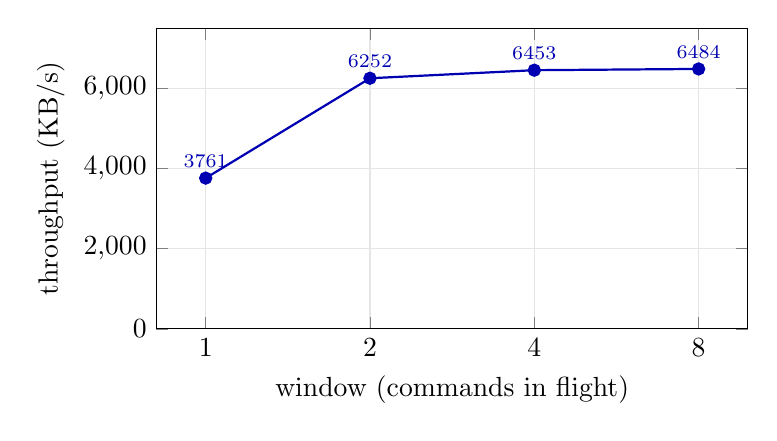
\begin{tikzpicture}
\begin{axis}[
  width=0.75\textwidth,height=5.4cm,
  xlabel={window (commands in flight)},ylabel={throughput (KB/s)},
  xtick={1,2,4,8},xticklabels={1,2,4,8},xmode=log,log basis x=2,
  ymin=0,ymax=7500,grid=both,grid style={black!10},
  every axis plot/.append style={thick},
  nodes near coords,point meta=explicit symbolic,
  nodes near coords style={font=\scriptsize,above}]
\addplot[blue!70!black,mark=*] coordinates {(1,3761)[3761] (2,6252)[6252] (4,6453)[6453] (8,6484)[6484]};
\end{axis}
\end{tikzpicture}
\caption{Measured effect of the window (data of Table~\ref{tab:window}).}
\end{figure}

\paragraph{What the window result shows.} Going from a window of one (stop and wait) to two raises the throughput by about two thirds, because the next command is sent while the board still works on the previous one. A window of four or eight adds almost nothing: with two commands in flight the link is already full. This is the evidence that the design of the command engine does what it was meant to do, and it also shows that the default of four is more than enough for this board. For CBC encryption, which has to run serially, the window cannot help, and the test's throughput for CBC is correspondingly lower.

\section{Cryptographic throughput}

\begin{table}[ht]
\centering
\begin{tabular}{lrr}
\toprule
Operation (1 MiB) & Board (MB/s) & Local CPU (MB/s) \\
\midrule
SHA-256 & 2.79 & 152.84 \\
AES-ECB & 4.22 & \\
AES-CTR & 4.21 & \\
AES-CBC (encrypt) & 2.70 & 180.04 \\
\bottomrule
\end{tabular}
\caption{Throughput from \code{afalg\_test bench}. Local figures vary between runs.}
\end{table}

\paragraph{Reading the numbers.}
\begin{itemize}
  \item ECB and CTR, which can be pipelined, reach about 4.2~MB/s, which is 65 percent of the transport ceiling. The rest of the time is spent in the board's AES engine and in copying.
  \item CBC encryption is about 2.7~MB/s, which is 64 percent of ECB. Each chunk waits for the previous one, so the window gives no benefit, and every chunk pays the full round trip.
  \item SHA-256 is as slow as CBC, 2.8~MB/s. Hashing cannot be split across commands in the same way because each \code{update} depends on the previous state, and the shash interface waits for each reply.
  \item A 64 byte hash takes about 0.62~ms, almost all of it fixed cost per round trip. Demo~5 shows that many concurrent callers can overlap those costs.
  \item The local CPU is roughly 55 to 140 times faster, depending on the run (the local figure was 153 to 394 MB/s in different runs). The project is a demonstration of mechanism.
\end{itemize}


\chapter{Problems met and lessons}\label{ch:lessons}

This chapter records the problems that shaped the final design. Each is a place where the first approach was wrong.

\section{Lost packets on the board}

The first version of the daemon read the endpoint in a loop. It worked when the PC sent one request at a time and failed under pipelining, with retries and almost no throughput. The cause lies in the board's USB controller. A packet that arrives while no read is queued can disappear. The fix was to keep many reads queued with asynchronous I/O (Section~\ref{ch:board}). The retransmission timer and the reply cache on the board were added at the same time, because even with the fix the protocol should tolerate loss.

\section{Replays after a module reload}

A reloaded module started its tag counter again and received old cached replies from the board. The symptom was wrong answers, not errors. The fix is the random starting tag.

\section{Retransmission must not repeat work}

Resending a command on timeout is only safe if executing it twice does no harm. Hashes with sessions and chained ciphers would be corrupted. The answer is the board's reply cache keyed by tag, which makes retransmission idempotent.

\section{GCM without kernel support}

The board kernel had no AEAD interface for AF\_ALG. A simple route would have been to rebuild the kernel. With no recovery path on the board, that risk was not accepted, so GCM was assembled in the daemon, using the hardware for the AES work. This also gave a worked example of how GCM is built from CTR and GHASH.

\section{Never kill the daemon while the gadget is bound}

Killing the daemon with the gadget bound hung the board's kernel twice. Every script now unbinds first. This is a recurring pattern in driver work: the order in which one tears things down matters as much as the order in which one sets them up.

\section{Disconnect while busy}

Pulling the cable while requests were in flight is the hardest case for a driver. The answer was reference counts on the board structure and on commands, a \code{dead} flag checked under the same lock as the queues, anchored URBs that can be cancelled together, and a failure work item that completes every pending request with an error. The unplug test repeats this in a loop.

\section{Keeping the algorithms registered}

Unregistering algorithms on disconnect made the crypto core warn when a program still held a socket. Leaving them registered, and failing with \code{-ENODEV} until a board returns, is the behaviour the core expects.

\section{Environmental limits}

A module must be built for the exact kernel it loads into. The module is unsigned, so a machine with Secure Boot enforcement will refuse it. Some distributions disable the AF\_ALG AEAD module, which the GCM tests need. The deployment script handles missing headers and tries to load the helper modules, and it reports clearly when loading fails.

\section{What the work shows}

\begin{itemize}
  \item A driver is mostly lifetime management. The crypto algorithms were the easy part. Making the structure survive a cable pull, a timeout, a module reload and a socket held open by a program took most of the code.
  \item The interface to a subsystem drives the design. Choosing the asynchronous crypto interfaces led directly to the command engine.
  \item Hardware has quirks that no documentation lists. The lost packet problem was found by measurement, not by reading.
  \item Testing against a reference is cheap and powerful. Comparing every output with the kernel's own implementation caught problems immediately and made later changes safe.
\end{itemize}

\chapter{Security considerations}\label{ch:security}

\section{What is protected and what is not}

A crypto accelerator moves secrets. The project is a driver exercise, and its security properties are limited, and it is useful to state exactly how.

\begin{table}[ht]
\centering
\begin{tabularx}{\textwidth}{lX}
\toprule
Asset & Exposure \\
\midrule
Keys & travel over the USB cable in clear with every cipher and HMAC command, and appear in the board's memory for the duration of the request \\
Plaintext and ciphertext & travel in clear over the cable in both directions \\
Command integrity & no authentication: a device on the cable that speaks the protocol can answer a request \\
Board identity & the host accepts any USB device with the right ids and interface class \\
\bottomrule
\end{tabularx}
\caption{Exposure of assets.}
\end{table}

The threat model is physical: anyone who can plug into or tap the USB cable, or who can attach a device that looks like the board, can read and alter the traffic. For a laboratory project this is acceptable. The report states it so no one mistakes the board for a trusted crypto device.

\section{What the code does for safety}

\begin{itemize}
  \item \textbf{Bounds checks everywhere.} Both sides check every length in a header against its limit and against the number of bytes received before using it. A malformed message cannot make either side read or write out of bounds.
  \item \textbf{Constant time tag comparison.} The daemon accumulates the xor of all tag bytes and tests the result once, so the time taken does not tell an attacker which byte first differed.
  \item \textbf{Authentication failure is an error, not output.} A failed GCM check produces no plaintext at all; the daemon returns \code{-EBADMSG} before copying any result.
  \item \textbf{Keys are not cached.} The board opens a transform per cipher request and closes it afterwards. The host copies the key only into the transform context, which is freed with the transform.
  \item \textbf{No secrets in scripts.} The deployment script takes the sudo password from an environment variable and passes it to \code{sudo -S} through the shell, so it never appears in the process list. Defaults for the board (an address and a known default password of the image) are overridable and apply only to a direct cable link.
  \item \textbf{Unsigned module.} The module is not signed. On a system that enforces signatures it will not load, which is the correct behaviour for such a system.
\end{itemize}

\section{What a production design would add}

\begin{itemize}
  \item an authenticated and encrypted channel between host and board, for example a key agreed at provisioning, so that traffic and keys are protected on the cable;
  \item key handles: keys loaded once onto the board and referred to by an id, so they do not travel with every request;
  \item device authentication, so the host accepts only the intended board;
  \item zeroing of key buffers on the host side after use, and use of the kernel's key retention services;
  \item rate limits and resource limits on the board for hash sessions, against a misbehaving host.
\end{itemize}


\chapter{Limitations and future work}

\begin{itemize}
  \item \textbf{Speed.} The accelerator is slower than the PC. A faster link or a faster board would change that, as would batching small requests.
  \item \textbf{Security of the link.} The USB link is not authenticated or encrypted. Anyone with physical access to the cable can read the data and the keys, which are sent with each request. A real product would protect the channel.
  \item \textbf{Key handling.} Keys travel with every command and are held in kernel memory. A design with keys stored on the device and referenced by handle would be safer.
  \item \textbf{Algorithms.} Only SHA-1, SHA-256, HMAC-SHA-256 and AES in four modes are offered. Other hashes, other modes and random number generation could be added with the same protocol.
  \item \textbf{GCM on the board.} Enabling AEAD in the board kernel would remove the software GHASH and allow the board's own GCM engine.
  \item \textbf{Automated testing without hardware.} Every functional test needs the real board. A mock of the daemon speaking the same protocol over a pipe would allow the suite to run in continuous integration.
  \item \textbf{Refactoring.} Several functions are long, notably the probe function in the module and the serving loop in the daemon. Splitting them is worth doing when a recoverable board is available for testing.
\end{itemize}

\chapter{Conclusion}

The project built a working USB device driver for Linux and the device it drives. The module registers real crypto algorithms with the kernel, so existing programs use the board without change. The board daemon turns a small ARM computer into a crypto peripheral, using its hardware engines through the kernel's own interface. The protocol is small, tagged and retransmitting, and the engine keeps several commands in flight. The result passes 690 checks against reference implementations on real hardware, with no errors or retries over tens of thousands of requests.

The work also shows how a driver sits between two worlds. On one side it speaks a hardware protocol, here USB bulk transfers with their packet rules. On the other side it implements a subsystem contract, here the asynchronous crypto API with its priorities, types and completion rules. Most of the effort went into the places where those two worlds disagree: timing, failure, ownership and teardown.

% ====================================================================
\appendix
\chapter{Command reference}
% ====================================================================

\section{Module parameters}

\begin{table}[ht]
\centering
\begin{tabularx}{\textwidth}{llXl}
\toprule
Name & Default & Meaning & Changeable \\
\midrule
\code{prio} & 50 & crypto API priority of all registered algorithms & at load \\
\code{window} & 4 & commands in flight per board, 1 to 8 & at run time \\
\code{chunk} & 16384 & bytes per cipher command, multiple of 16, up to 32768 & at run time \\
\bottomrule
\end{tabularx}
\caption{Module parameters of \code{bbcrypto}.}
\end{table}

\section{Registered algorithms}

\begin{table}[ht]
\centering
\begin{tabular}{ll}
\toprule
Generic name & Driver name \\
\midrule
\code{sha1} & \code{sha1-bbcrypto}, \code{sha1-async-bbcrypto} \\
\code{sha256} & \code{sha256-bbcrypto}, \code{sha256-async-bbcrypto} \\
\code{hmac(sha256)} & \code{hmac-sha256-bbcrypto}, \code{hmac-sha256-async-bbcrypto} \\
\code{ecb(aes)} & \code{ecb-aes-bbcrypto} \\
\code{cbc(aes)} & \code{cbc-aes-bbcrypto} \\
\code{ctr(aes)} & \code{ctr-aes-bbcrypto} \\
\code{gcm(aes)} & \code{gcm-aes-bbcrypto} \\
\bottomrule
\end{tabular}
\caption{Algorithms provided by the module.}
\end{table}

\section{Common commands}

\begin{lstlisting}[style=shell]
make deploy HOST=user@machine       # build, install, load and test remotely
make install-board                  # copy daemon and services to the board
sudo modprobe bbcrypto prio=400     # make plain names use the board
cat /sys/bus/usb/drivers/bbcrypto/*/stats
sudo tests/afalg_test               # full functional suite
sudo tests/afalg_test unplug        # device removal test
python3 demos/4_priority.py         # who answers a plain sha256 request
\end{lstlisting}

\chapter{Message sequence of one request}

Figure~\ref{fig:seq} shows one 16 KiB CBC decrypt chunk, including a lost reply and the retry that follows.

\begin{figure}[ht]
\centering
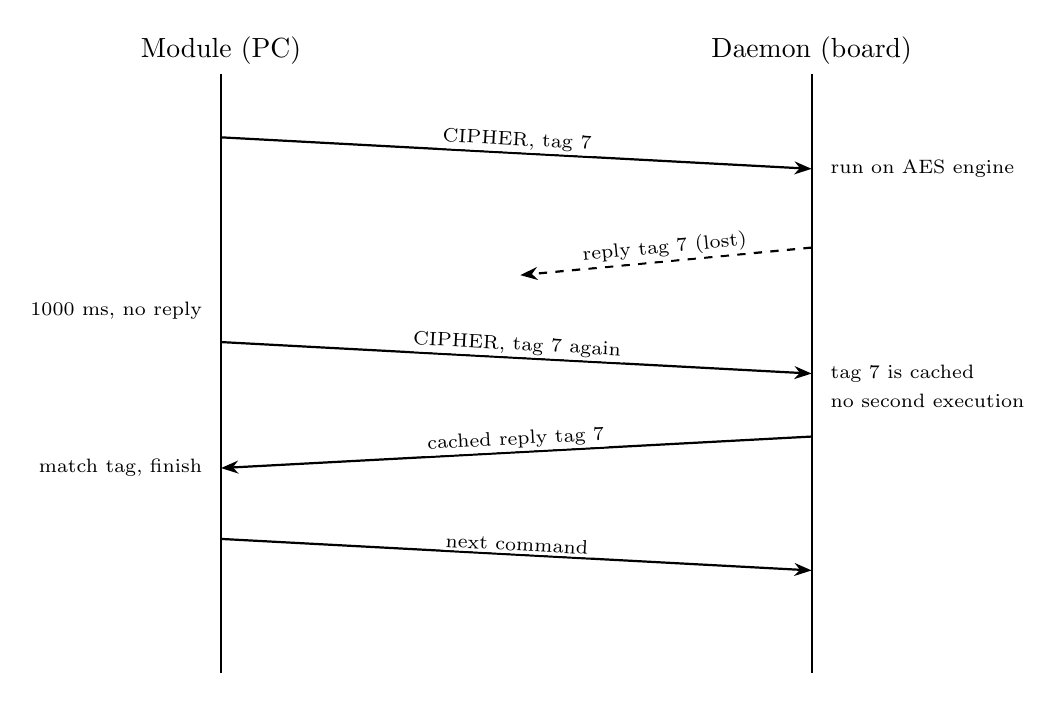
\begin{tikzpicture}[x=1cm,y=1cm]
  \draw[thick] (0,0) -- (0,-7.6); \node[above] at (0,0) {Module (PC)};
  \draw[thick] (7.5,0) -- (7.5,-7.6); \node[above] at (7.5,0) {Daemon (board)};
  \draw[arr] (0,-0.8) -- node[lbl,above,sloped]{CIPHER, tag 7} (7.5,-1.2);
  \node[lbl,anchor=west] at (7.7,-1.2) {run on AES engine};
  \draw[arr,dashed] (7.5,-2.2) -- node[lbl,above,sloped]{reply tag 7 (lost)} (3.8,-2.55);
  \node[lbl,anchor=east] at (-0.2,-3.0) {1000 ms, no reply};
  \draw[arr] (0,-3.4) -- node[lbl,above,sloped]{CIPHER, tag 7 again} (7.5,-3.8);
  \node[lbl,anchor=west] at (7.7,-3.8) {tag 7 is cached};
  \node[lbl,anchor=west] at (7.7,-4.15) {no second execution};
  \draw[arr] (7.5,-4.6) -- node[lbl,above,sloped]{cached reply tag 7} (0,-5.0);
  \node[lbl,anchor=east] at (-0.2,-5.0) {match tag, finish};
  \draw[arr] (0,-5.9) -- node[lbl,above,sloped]{next command} (7.5,-6.3);
\end{tikzpicture}
\caption{A retransmission. The board answers the repeated tag from its reply cache.}\label{fig:seq}
\end{figure}

\chapter*{Glossary}\addcontentsline{toc}{chapter}{Glossary}

\begin{description}
  \item[AEAD] authenticated encryption with associated data. GCM is an AEAD mode.
  \item[AF\_ALG] the socket family through which user programs reach the kernel crypto API.
  \item[AIO] the kernel's asynchronous I/O interface. The daemon uses it to keep reads queued.
  \item[Anchor] a USB core object that groups the URBs of a device so they can be cancelled together.
  \item[Bulk transfer] USB transfer type for large, loss-free data without timing guarantees.
  \item[Completion] a kernel object a thread can sleep on until another context signals it.
  \item[ConfigFS] a file system through which user space creates kernel objects, used here to build gadgets.
  \item[Endpoint] one data pipe of a USB interface.
  \item[FunctionFS] a gadget function implemented in user space through files for each endpoint.
  \item[Gadget] a USB device implemented by a Linux system.
  \item[GCM] Galois/Counter Mode, an AEAD mode for block ciphers.
  \item[GHASH] the polynomial hash over $GF(2^{128})$ used by GCM for authentication.
  \item[Interface] one function of a USB device. Drivers bind to interfaces.
  \item[kbuild] the kernel's build system for modules.
  \item[kref] kernel reference counter.
  \item[MUSB] the USB controller design used in the AM335x.
  \item[Probe] the driver function called when a matching device appears.
  \item[Scatterlist] a list of memory fragments that together form one logical buffer.
  \item[Spinlock] a lock that busy waits, usable in interrupt context.
  \item[Tag (protocol)] a number that identifies a command so a reply can be matched to it.
  \item[Transform] a crypto API object that holds an algorithm and its key.
  \item[UDC] USB device controller, the hardware that makes a board act as a device.
  \item[URB] USB request block, the unit of USB I/O in the kernel.
  \item[Window] the maximum number of commands in flight at once.
  \item[Workqueue] a kernel facility that runs functions later in process context.
\end{description}

\begin{thebibliography}{99}
\bibitem{ldd3} J.~Corbet, A.~Rubini, G.~Kroah-Hartman, \emph{Linux Device Drivers}, 3rd ed., O'Reilly, 2005.
\bibitem{kdocs} The Linux kernel documentation, \url{https://docs.kernel.org}, in particular the sections on the driver API, USB, the crypto API and gadget FunctionFS.
\bibitem{usb2} Universal Serial Bus Specification, Revision 2.0, USB Implementers Forum, 2000.
\bibitem{fips180} NIST, FIPS PUB 180-4, \emph{Secure Hash Standard}, 2015.
\bibitem{fips197} NIST, FIPS PUB 197, \emph{Advanced Encryption Standard}, 2001.
\bibitem{sp80038a} NIST, SP 800-38A, \emph{Recommendation for Block Cipher Modes of Operation}, 2001.
\bibitem{sp80038d} NIST, SP 800-38D, \emph{Recommendation for Block Cipher Modes of Operation: Galois/Counter Mode (GCM) and GMAC}, 2007.
\bibitem{rfc2104} H.~Krawczyk, M.~Bellare, R.~Canetti, RFC 2104, \emph{HMAC: Keyed-Hashing for Message Authentication}, 1997.
\bibitem{am335x} Texas Instruments, \emph{AM335x Sitara Processors Technical Reference Manual}.
\end{thebibliography}


\end{document}
